  %%%%%%%%%%%%%%%%%%%%%%%%%%%%%%%%%%%%%%%%%%%%%%%%%
%------ LaTeX-Template für Abschlussarbeiten, Prof. Thomas Görne, Dezember 2012 --------
%%%%%%%%%%%%%%%%%%%%%%%%%%%%%%%%%%%%%%%%%%%%%%%%%

%---- Header (mit Formateinstellugen) laden, Inputencoding prüfen ------

%%%%%%%%%%%%%%%%%%%%%%%%%%%%%%%%%%%%%%%%%%%%%%%%%
%---- LaTeX-Header fuer Abschlussarbeiten, Prof. Thomas Goerne, Dez. 2012/Aug. 2013 ----
%%%%%%%%%%%%%%%%%%%%%%%%%%%%%%%%%%%%%%%%%%%%%%%%%

\documentclass[12pt,paper=A4,pointlessnumbers,bibtotoc,liststotoc,DIV=11,BCOR=1mm,halfparskip]{scrreprt}
% BCOR ist die Bindekorrektur (verlorener Rand am linken Blattrand)! Wert haengt von der Art der Heftung ab!!
% DIV ist eine Satzspiegeleinstellung von KOMA-Script / sccreprt.
\hyphenpenalty = 1000
\usepackage[a4paper,
left=2.5cm, right=2.5cm,
top=2.5cm, bottom=2.5cm]{geometry}

\pagestyle{headings}
\usepackage[utf8]{inputenc}
\usepackage[T1]{fontenc} % Font Encoding fuer europaeische Schriften mit Umlauten (Unterstuetzung der Worttrennung)
\usepackage{lmodern} % PostScript-Varianten der TeX Computer Modern-Schriften laden
\usepackage[english,ngerman]{babel} % Spracheinstellungen fuer Englisch und Neudeutsch laden
\usepackage[autostyle=true,german=quotes]{csquotes}
\usepackage{times}                                     % Schriften Paket
\usepackage{array,ragged2e}                            % Wichtig für Abstandsformatierung
\usepackage{cmbright}                                  % serifenlose Schrift als Standard + alle für TeX
                                                       % benötigten mathematischen Schriften einschließlich der AMS-Symbole
\usepackage[scaled=.90]{helvet}                        % skalierte Helvetica als \sfdefault
\usepackage{courier}                                   % Courier als \ttdefault
\usepackage[automark]{scrpage2}                        % Anpassung der Kopf- und Fußzeilen
\usepackage{xspace}                                    % Korrekter Leerraum nach Befehlsdefinitionen
\usepackage[onehalfspacing]{setspace}                                % 1.5 zeilen abstand

\usepackage{graphicx} % Grafikeinbindung (fuer .JPG, .JPEG, .PNG und .PDF, falls pdflatex benutzt wird)
\usepackage[table]{xcolor} % ermoeglicht farbige Schrift und farbige Tabellenzeilen
\definecolor{black}{gray}{0} % Umdefinition der Farbe black, falls noetig (0=schwarz, 1=weiss)
\definecolor{dblue}{rgb}{0.1,0.2,0.6} % Dunkelblau, fuer Hyperlinks
\definecolor{lgray}{gray}{0.9} % Hellgrau, fuer Tabellen (0=schwarz, 1=weiss)

\usepackage[final]{pdfpages}                           % include pages of external PDF documents
\usepackage{tabularx}                                  % Spaltenbreite bis zur Seitenbreite dehnen

\usepackage{booktabs} % fuer schoene Tabellen

\usepackage[round,authoryear]{natbib} % Literaturverweise mit Name/Jahreszahl in runden Klammern
\bibpunct[:\,]{(}{)}{,}{a}{}{,~}  % Feinformatierung der Natbib-Zitierweise

\usepackage[hyphens]{url}
\usepackage[colorlinks=true,linkcolor=dblue,citecolor=dblue,urlcolor=dblue]{hyperref}
% die Pakete url und hyperref ermoeglichen anklickbare URLs im Quellenverzeichnis in definierter Farbe,
% sie ermoeglichen den Zeilenumbruch bei langen URLs, und sie erzeugen Hyperlinks (Farbe s.o.)
% zwischen Quellenverweis und Quellenverzeichnis sowie zwischen label und ref im PDF-Dokument

% Fonteinstellungen fuer Bildunterschriften: Unterschrift serifenlos, "Abbildung" fett (bfseries = bold face series)
\setkomafont{captionlabel}{\sffamily\bfseries}
\setkomafont{caption}{\sffamily}

\usepackage{makeidx}
\usepackage[cache=false]{minted}
\setminted{fontsize=\small,baselinestretch=1}
\renewcommand{\listingscaption}{Quellcode}
\renewcommand{\listoflistingscaption}{Quellcode Verzeichnis}
\usepackage{multirow}
\usepackage[xindy]{glossaries}
\newglossaryentry{databinding}
{
  name = Databinding,
  description = {  Eine Teschnik, welche die Benutzeroberfläche der App mit den dort angezeigten Daten verbindet und synchronisiert }
}

\newglossaryentry{json}
{
  name = JSON,
  description = { Javascript Object Notation. \url{http://json.org/} }
}

\newglossaryentry{di}
{
  name = Dependency Injection,
  description = { Ein Entwurfsmuster der objektorientierten Programmierung, bei dem Abhängigkeit zwischen Objekten erst zur Laufzeit hergestellt werden }
}

\newglossaryentry{ng-directive}
{
  name = AngularJS Direktive,
  description = { Marker auf dem DOM Element, welcher dem AngularJS Renderer mitteilt spezifisches Verhalten an das DOM Element zu binden. \url{https://docs.angularjs.org/guide/directive}}
}

\newglossaryentry{ng-service}
{
  name = Angular Service,
  description = { Ersetzbare Objekte, welche zusammengebunden werden um Code zu organisieren und zwischen Modulen zu teilen. \url{https://docs.angularjs.org/guide/services}}
}

\newglossaryentry{ng-factory}
{
  name = Angular Factory,
  description = { Komponenten, welche Services erzeugen. \url{https://docs.angularjs.org/guide/providers\#factory-recipe}}
}


\newglossaryentry{pug}
{
  name = Pug,
  description = { Javascript HTML Template Engine. \url{https://pugjs.org/} }
}

\newglossaryentry{transpiler}
{
  name = Transpiler,
  description = {Source to Source Compiler}
}

\newglossaryentry{localstorage}
{
  name = LocalStorage,
  description = { HTML5 Web Storage Schnittstelle. \url{https://www.w3schools.com/html/html5\_webstorage.asp} }
}


\newglossaryentry{webpack}
{
  name = Webpack,
  description = { Javascript module bundler. \url{https://webpack.js.org/}}
}

\newglossaryentry{es2016}
{
  name = ES2016,
  description = { Spezifische Version des ECMAScript standardisierten Sprachkerns von JavaScript. \url{http://www.ecma-international.org/ecma-262/7.0/}}
}

\newglossaryentry{sass}{
  name = SASS,
  description = { Stylesheet-Sprache, die als CSS-Präprozessor, mit Variablen, Schleifen und vielen anderen Funktionen, die Cascading Style Sheets (CSS) nicht mitbringen, die Erstellung von CSS vereinfacht und die Pflege großer Stylesheets erleichtert }
}

\newglossaryentry{jwt}
{
  name = JWT,
  description = {Jason Web Token. JSON Web Tokens sind eine offene Industriestandard RFC 7519 Methode zur sicheren Representierung von Forderungen zwischen zwei Parteien }
}

\newglossaryentry{promise}
{
  name = Promise,
  description = {Eine Repräsentation einer eventuellen Ausführung einer asynchronen Operation}

}

\makeglossaries
\usepackage[xindy]{imakeidx}
\makeindex


%------------------------------------------------------------------------------------------------------------------
%------ Eigenstaendigkeitserklaerung im gerahmten Kasten (parbox in einer framebox) ------
%------------------------------------------------------------------------------------------------------------------

\newcommand{\eigen}{
\setlength{\fboxsep}{2ex}
\setlength{\fboxrule}{0.8pt}
% Einstellungen fuer Rahmenabstand und Rahmendicke der Framebox
\begin{center}
  \fbox{
    \parbox{0.8\linewidth}{
    Ich versichere, die vorliegende Arbeit selbstst\"andig ohne fremde Hilfe verfasst
    und keine anderen Quellen und Hilfsmittel als die angegebenen benutzt zu haben.
    Die aus anderen Werken w\"ortlich entnommenen Stellen oder dem Sinn nach
    entlehnten Passagen sind durch Quellenangaben eindeutig kenntlich gemacht.
    \par\bigskip\bigskip\bigskip\bigskip
    \hspace*{0.8cm}Ort, Datum \hfill \vorname~\nachname\hspace*{0.8cm}
    }
  }
\end{center}
}

%%%%%%%%%%%%%%%%%%%%%%%%%%%%%%%%%%%%%%%%%%%%%%%%%

%\usepackage[applemac]{inputenc} % Inputencoding für Mac
%\usepackage[latin1]{inputenc} % Inputencoding für PC/Win
\usepackage[utf8]{inputenc} % Inputencoding, universell
%\usepackage[utf8x]{inputenc} % Inputencoding, universell


%------------------------ Titelblatt-Layout laden ----------------------------------

\input{hawmt-bachelor-titelblatt}
%\input{hawmt-master-titelblatt}

%---------------------------- Titeldefinitionen --------------------------------------

\newcommand{\vorname}{Anastasia}
\newcommand{\nachname}{Stieb}
\newcommand{\matrikelnummer}{Matrikel-Nr. 2023959}

\newcommand{\titel}{Software Architektur Elemente des JavaScript Clients in einer Single Page Webapplikation \\[0.2ex]
				\Large am Beispiel einer Fotoverwaltungssoftware}

\newcommand{\erstpruef}{Prof. Dr. Andreas Plaß}
\newcommand{\zweitpruef}{Prof. Dr. Torsten Edeler}

%\date{vorläufige Fassung vom \today}   % praktisch für Vorab-Versionen.
\date{\sffamily Hamburg, 15. 7. 2021}  % Abgabedatum!

%--------------------------------------------------------------------------------------
%----------------------------- hier gehts los! --------------------------------------
%--------------------------------------------------------------------------------------

\begin{document}
\selectlanguage{ngerman}
\maketitle           % Titelseite erzeugen
\newpage

%------------ Zusammenfassung / Abstract ------------------

\thispagestyle{empty}
\selectlanguage{english}
\subsection*{Title of Paper}
Software Architecture Elements of a JavaScript Client in a Single Page Webapplication

\subsection*{Keywords}


\subsection*{\centering\abstractname}
This bachelor thesis focuses on the realisation of a potentially user interaction rich, similar to native clients in a webapplication by implementing a photo management software as example.


\selectlanguage{ngerman}
\subsection*{Thema der Arbeit}
Software Architektur Elemente des JavaScript Clients in einer Single Page Webapplikation


\subsection*{Stichworte}
\subsection*{\centering\abstractname}
Diese Bacherlorarbeit befasst sich mit der Realisierung eines potentiell an Benutzerinteraktionen reichen, nativ ähnlichen Clients einer Webanwendung am Beispiel der Implementierung einer Fotoverwaltungssoftware.

\newpage


\tableofcontents % Inhaltsverzeichnis erzeugen
\newpage


%--------------------------- Text -------------------------------
\chapter{Einleitung}

\section{Motivation}

 ``There is no cloud it's just someone else's Computer'' - eigentlich ein ganz
 triviales Statement, doch es wurde zu einem Internetphänomen, auch ``Meme''
 genannt, weil die Webindustrie es geschafft hat, für einen Benutzer
 transparent werden zu lassen, dass hinter so manchem Dienst sich in der Realität ein ganzes Rechenzentrum befindet.


Die große Rechenpower, die von jedem Ort, jeder Zeit verfügbar ist, machte auch
eine Breite verschiedener portabler Anzeigegeräte ubiquitär. Die Werbemarketing
Spezialisten sprechen von einem ``Second Screen'', aber in Wirklichkeit ist
jedes andere internetfähige Gerät gemeint, welches parallel zum laufenden
Fernsehprogramm genutzt wird und bei so manchem Anwender ist die Zahl
längst über zwei.


Viele kleine Applikationen sollen diese portablen Geräte zu intelligenten
persönlichen Assistenten machen, jedoch ist immer noch das beliebteste Programm
der Webbrowser. (App fatigue Artikel zitieren)


Ebenfalls hat sich an den Grundprotokollen, die das World Wide Web seit 1991 zu
Nutze macht nicht viel geändert. Obwohl ganz


%%% Local Variables:
%%% TeX-master: "../master"
%%% End:
\chapter{Analyse}
\label{sec:analysis}

\section{Einleitung}

In dem Kapitel \hyperref[sec:motivation]{Motivation} wurde geschildert, dass eine Web-Fotoverwaltungssoftware als Exempel für die Zielsetzungen dieser Arbeit dienen wird. Nun soll analysiert werden, welche Realanforderungen notwendig sind, um den zuvor definierten \hyperref[sec:zielsetzung]{Zielsetzungen} gerecht zu werden.

\section{User Experience}

Folgend werden Anforderungen beschrieben, die sich mit dem Nutzungserlebnis und der visuellen Gestaltung der Applikation befassen.

\subsection{Schnelles Feedback}

Die Hauptanforderung an die Webanwendung besteht darin, dem Benutzer das an eine native Applikation angelehnte Nutzungserlebnis zu gewährleisten. Die bei einer
klassischen Webanwendung entstehenden Ladezeiten, welche nach jeder Benutzerinteraktion durch das erneute Laden und Darstellen des gesamten Inhaltes
auftreten, sollen vermieden werden.

\subsection{Flaches Design}

Das Benutzerinterface der Anwendung soll unter Anwendung der Paradigmen vom flachen Design minimalistisch, jedoch mit klar erkennbaren Aktionsaufrufen, gestaltet werden.

\subsection{Responsive Design}

Die Webanwendung soll sich auf potentiell unterschiedliche Displaygrößen anpassen. Das Benutzerinterface soll dabei nicht komplett für jede mögliche Abstufung der Displaygröße neu gestaltet werden. Für das Layout sollen Regeln verwendet werden, die es dem gleichen Interface erlauben, seine Elemente bei schrumpfender bzw. wachsender Größe neu zu positionieren.

\subsection{Fotozentrierung}
\label{sec:spec:photo_centering}

Ein besonderes Unterproblem der Adaptierung an verschiedene Gerätedisplays ist die Fotobetrachtung. Hier sind sowohl die Auflösung des Fotos als auch des Displays für die Software nicht zu Implementierungszeit, sondern erst zur Laufzeit bekannt. Um das Foto in der Gesamtheit auf einem beliebigen Display zu betrachten, soll es zur Laufzeit sowohl in der Detailansicht als auch innerhalb seines Platzhalters in der Gesamtübersicht zentriert werden.

\section{User Stories}

In diesem Unterkapitel werden die einzelnen Features der Beispiel-Applikation definiert.

\subsection{Authentifizierung}
\label{sec:spec:authentication}

Die Fotosoftware soll den Benutzern nur anhand einer Benutzerkennung und eines Passworts den Zugang gewähren.

\subsection{Navigation Menü}
\label{sec:spec:menu}

Der Benutzer soll im Stande sein zwischen den Hauptfunkionen der Anwendung aus jedem beliebigen Unterbereich zu navigieren.

\subsection{Foto Galerie}
\label{sec:spec:photo_gallery}

Dem Benutzer soll eine Auflistung seiner gespeicherten Fotos dargestellt werden.

\subsection{Paginierung/Nachladen der Fotos}
\label{sec:spec:pagination}

Falls sich sehr viele Fotos in der \hyperref[sec:spec:photo_gallery]{Foto Galerie} befinden, sollen diese nicht im selben Augenblick geladen werden, damit die Anwendung nicht überlastet wird. Stattdessen soll zuerst eine bestimmte Anzahl der Fotos dargestellt werden und es anschließend dem Benutzer ermöglicht werden, weitere Bilder stapelweise nachzuladen.

\subsection{Foto Freitext Suche}
\label{sec:spec:photo_search}

Der Benutzer soll in Beschreibungen und Namen nach seinen Fotos durch Eingabe von Freitext suchen können. Das Resultat der Suche soll ebenfalls wie die Fotogalerie paginiert werden.

\subsection{Fotos nach Erstellungsmonat gruppieren}
\label{sec:spec:photo_groups}

Dem Benutzer soll ermöglicht werden, die Fotos nach Erstellungsmonat gruppiert zu betrachten. Die Darstellung der Monatsgruppen erfolgt in absteigender Reihenfolge.

\subsection{Foto Details}
\label{sec:spec:photo_details}

Der Benutzer soll in der Lage sein, Fotos mit Metadaten wie Name und Beschreibung zu annotieren. Bei der Auswahl eines einzelnen Fotos in der Galerie sollen diese annotierten Fotoinformationen veranschaulicht werden.

\subsection{Foto Großansicht}

Dem Benutzer soll ermöglicht werden, ein bestimmtes Foto in der vollständiger Größe zu betrachten.

\subsection{Foto Slider}
\label{sec:spec:photo_slider}

Wenn der Benutzer die Detailansicht eines Fotos aus der Galerie auswählt, soll es ihm ferner möglich sein aus der Detailansicht zum nächsten oder dem vorherigen Foto zu navigieren.

\chapter{Grundlagen}

\section{Client/Server Model}
\label{sec:client_server}

Webanwendungen sind eine erweiterte Form von normalen Webseiten und funktionieren nach den selben Prinzipien des World Wide Webs. Diesen liegt wiederum das Client-/Server-Model zu Grunde.

Der Client ist ein Programm des Benutzers und ist dafür zuständig, den Inhalt der Applikation oder Webseite auf dem Bildschirm in benutzerfreundlicher Art und Weise zu verarbeiten. Ein solcher typischer Client ist der Web Browser.

Der Inhalt selbst befindet sich auf einem entfernten Rechner, genannt der Server. Server verarbeiten eingehende Anfragen der Clients nach Inhalten und liefern eine Kopie dieser Inhalte aus. Der heruntergeladene Inhalt kann schließlich vom Client angezeigt werden.

Die Fachbezeichnung für den remote Inhalt ist Ressource. Ressourcen können aus Bildern, Videos, Webseiten und andere Dateien bestehen. Aber wie am Anfang angedeutet, sind Ressourcen nicht nur auf Dateien und Webseiten beschränkt. Sie können auch in Form vom Software vorkommen, welche es z.B. erlauben, Aktien zu handeln oder Videospiele zu spielen. Ressourcen werden dabei durch einen eindeutigen Bezeichner - die URL - identifiziert.

Ein simples Diagramm, wie Client und Server interagieren können, sieht wie folgt aus:

Historisch ergeben, nutzen Client und Server das Kommunikationsprotokoll HTTP für die Kommunikation untereinander. Diese Übertragung ist zustandslos. Diese Eigenschaft wurde absichtlich konzipiert, um die Protokoll-Implementierung einfach zu halten und um Serverressourcen zu sparen. Der Server muss dabei keine Benutzerinformation zwischen den Anfragen merken. Im Fehlerfall muss ebenfalls nichts aufgeräumt werden. Die beiden Gründe machen HTTP zu einem sehr belastbaren Protokoll, aber auch gleichzeitig zu einem schwierigen Protokoll, um zustandsbehaftete Webanwendungen zu implementieren.

\cite[Background]{Parikh:2015} beschreibt das Problem wie folgt:

"When you go to Facebook, for example, and log in, you expect to see the internal Facebook page. That was one complete request/response cycle. You then click on the picture -- another request/response cycle -- but you do not expect to be logged out after that action. If HTTP is stateless, how did the application maintain state and remember that you already input your username and password? In fact, if HTTP is stateless, how does Facebook even know this request came from you, and how does it differentiate data from you vs. any other user? There are tricks web developers and frameworks employ to make it seem like the application is stateful..."

D.h, dass es eine Reihe von verschiedenen Techniken gibt, welche auf Anwendungsebene realisiert werden müssen, um Zustandshaftigkeit in einem zustandslosen Protokoll zu gewährleisten.

Vgl. \cite[Background]{Parikh:2015}, \cite{Culloca:2006}

\section{HTTP}

In \ref{sec:client_server} wurde erwähnt, dass im World Wide Web das Kommunikationsprotokoll HTTP verwendet wird. Ein Protokoll zeichnet sich zunächst durch 3 grundlegende Eigenschaften aus:

\begin{itemize}
\item Syntax - Datenformat und Kodierung
\item Semantik - Steuerungsinformation und Fehlerbehandlung
\item Zeitablauf - Geschwindigkeitsanpassung und Reihenfolge
\end{itemize}

\cite{Dubost:2012} zeigt, dass Kommunikationsprotokolle nicht nur ein künstliches Konstrukt sind, sondern auch aus der realen Welt stammen:

"When two people meet, they engage using a communication protocol: for example, in Japan, a person will make a specific gesture with the body. One such gesture is a bow, which is the syntax used for the interaction. In Japanese customs, the gesture of the bow (among others) is associated with the semantics of greeting someone. Finally, when one person bows to another person, a sequence of events has been established between the two in a specific timing."

Weiterhin beschreibt \cite{Dubost:2012}, dass in einem Online-Kommunikationsprotokoll die gleichen Elemente vorkommen: die Syntax - die Abfolge von Zeichen, etwa Bezeichnern, die für das Schreiben des Protokolls verwendet werden; die Semantik - die Bedeutung, die mit diesen Bezeichnern assoziiert wird; und schließlich der Zeitablauf - eine vorgegebene Reihenfolge, in der Client und Server diese Bezeichner austauschen.

HTTP ist dabei ein sog. Application Level Protocol, d.h, dass es in der Abstraktionsebene höher angesiedelt ist. Es setzt wiederum auf eine Reihe weiterer Protokolle auf, welche sich etwa um die Übertragung der eigentlichen Datenpakete oder die physikalische Übertragung der elektrischen Signale kümmern. HTTP selbst beschreibt hingegen die Bedeutung und das Format der gesamten übertragenen Nachricht.

Folgend ist eine HTTP GET Anfrage aufgelistet:

\begin{listing}[H]
\begin{minted}{http}
GET / HTTP/1.1
Host: www.opera.com
User-Agent: Opera
\end{minted}
\caption{HTTP GET Request}
\end{listing}

Diese Nachricht spezifiziert, dass der Client eine Ressource erhalten möchte.
Die Ressource, die der Client erhalten möchte, befindet sich im root-Verzeichnis.
Die Übertragung soll mittels HTTP version 1.1 stattfinden. Der Client versucht eine spezifische Webseite zu erreichen, die sich unter der URL \emph{www.opera.com}befindet. Ferner teilt der Client einen sog. HTTP Header, namens \emph{User-Agent} Informationen über das Programm, welches für die Kommunikation verwendet wurde.

Eine Antwort vom Server könnte dabei wie folgt aussehen:

\begin{listing}[H]
\begin{minted}{http}
HTTP/1.1 200 OK
Date: Wed, 23 Nov 2011 19:41:37 GMT
Server: Apache
Content-Type: text/html; charset=utf-8
Set-Cookie: language=none; path=/; domain=www.opera.com;
  expires=Thu, 25-Aug-2030 19:41:38 GMT
Set-Cookie: language=en; path=/; domain=.opera.com;
  expires=Sat, 20-Nov-2030 19:41:38 GMT
Vary: Accept-Encoding
Transfer-Encoding: chunked

<!DOCTYPE html>
<html lang="en">
…
\end{minted}
\caption{HTTP GET Response}
\end{listing}

Der Server antwortet, dass er das Protokoll HTTP Version 1.1 versteht. Die Anfrage war erfolgreich und wurde daher mit dem Response Code 200 sowie einer verständlichen Annotation \textit{OK} versehen. Anschließend wird eine Reihe weiterer HTTP Header gesendet, welche beschreiben, wie die Nachricht verstanden werden soll. Und letzendlich wird der Inhalt der Ressource - hier ein HTML Dokument - in den Rumpf (body) der Nachricht eingefügt.

Weitere HTTP-Methoden sind: OPTIONS, GET, HEAD, POST, PUT, DELETE, TRACE, CONNECT.
Jede von denen hat eine unterschiedliche Rolle. Siehe \cite[Kap. 4]{Fielding:2014}. 

Vgl. \cite{Dubost:2012}

\section{Serverseitige Webanwendungen}

\subsection{Grundprinzip}

Als das World Wide Web geboren wurde, existierte nur ein Webserver und ein Webclient. Dieser Webserver namens httpd war nur in der Lage, statische Ressourcen wie Bilder und Dokumente auszuliefern. Schon bald jedoch machte der Überfluss an Online-Ressourcen Suchmaschinen notwendig. Das bedeutete, dass Benutzer in der Lage sein mussten, Daten, wie den Suchbegriff, an den Server abzuschicken und der Server seinerseits im Stande sein sein musste, diese Daten zu verarbeiten und dynamisch entsprechende Inhalte zu liefern.

Hierfür wurde das Common Gateway Interface (CGI) spezifiziert. Es entwickelte sich zum Standard, um externe Applikationen mit Webservern zu verbinden und um dynamische Information zu generieren. Ein CGI Programm kann beinahe in jeder Programmiersprache implementiert werden. Es muss nur die Fähigkeit besitzen, sein vom STDIN zu lesen und auf STDOUT zu schreiben.

Folgend ist ein exemplarisches CGI "Hello World" Programm dargestellt. Ein Benutzer namens Doug gibt seinen Namen ein, welcher vom Webserver ausgegeben werden soll. Dabei generiert sein Webclient einen HTTP GET Request an folgende URL:

\begin{minted}{http}
http://example.com/cgi-bin/hello.pl?username=Doug
\end{minted}

Wenn der Webserver diese Anfrage bekommt, weiß er, wie er die URL in zwei Teile trennt: den Pfad zu dem CGI Perl Programm \emph{hello.pl} und den Teil mit der Benutzereingabe (username=Doug, genannt QUERY\_STRING). Er leitet also diese Anfrage über STDIN an das \emph{hello.pl} Script weiter. Die Aufagbe des Scriptes ist nun, den QUERY\_STRING nach dem Schlüssel \emph{username} zu parsen und dessen Wert über SDTOUT auszugeben. Der Webserver wird wiederum diese Ausgabe an den Client weiterleiten. Das Beispiel "Hello user" Programm ist in \ref{lst:hello_pl} abgebildet.

\begin{listing}[H]
\begin{minted}{perl}
  #!/usr/bin/perl

  use CGI qw(:standard);
  my $username = param('username') || "unknown";

  print "Content-type: text/plain\n\n";
  print "Hello $username!\n";
\end{minted}
\caption{"Hello user" CGI script}
\label{lst:hello_pl}
\end{listing}

Ein solches serverseitiges Programm generiert für gewöhnlich dynamische Inhalte, indem es die Information dafür aus einer Datenbank bezieht. Heutige serverseitige Webanwendungen nutzen weiterhin entweder eine Weiterentwicklung der CGI Schnittstelle oder ein ähnliches Prinzip.

Vgl. \cite[Kap. 1.1]{Bekman:2003}

Im Kapitel \ref{sec:client_server} wurde auf die Diskrepanz hingewiesen, dass HTTP ein zustandsloses Protokoll ist, eine Webanwendung jedoch Zustandshaftigkeit benötigt, um Benutzersitzungen, etwa Besuch und Einkauf in einem Webshop, auseinanderzuhalten. Eine solche Session kann von dem Client und Server Programm
künstlich aufrecht erhalten werden.

Dabei generiert das serverseitige Programm einen Session-Identifier beim ersten Besuch des Benutzers und sendet es an den Client. Der Client wiederum sendet diese  ID bei jeder weiteren Anfrage an den Server mit. Ein Mechanismus für die Benutzersessions im Web ist das Setzen von HTTP-Cookies, welche dann automatisch bei den nachfolgenden Anfragen angehängt werden. Weitere manuelle Möglichkeiten sind  Übertragung mittels custom HTTP Header oder Umwandeln der URLs durch das Anhängen des zusätzlichen \emph{session\_id} Parameters.

Siehe \cite[Stateful Web Applications]{Parikh:2015}

\subsection{Architektur}

In objektorientierter Software ist für die Erstellung von graphischen Anwendungen das Model-View-Controller Pattern vorherrschend.

Galilio schreibt: "Mit Model-View-Controller (MVC) wird ein Interaktionsmuster in der Präsentationsschicht von Software beschrieben. MVC ist wohl einer der schillerndsten Begriffe im Bereich der objektorientierten Programmierung. Viele Varianten haben sich herausgebildet, teilweise einfach aufgrund eines falschen Verständnisses des ursprünglichen MVC-Musters, teilweise als Weiterentwicklung oder Anpassung an neue Anwendungsfälle."

Unabhängig von der jeweiligen Abwandlung des MVC Pattern gilt, dass der Controller für Benutzereingaben, das Model für den Zustand und der View für das Darstellen dieses Zustands verantwortlich ist. Vgl. Galilio  8.2.3

Serverseitige Webanwendungen interpretieren MVC wie folgt. Benutzerinteraktionen führen weitgehend zu Anfragen einer komplett neuen Ressource, e.g:

\begin{minted}{http}
GET http://example.com/articles
GET http://example.com/articles/1
GET http://example.com/articles/1/comments
\end{minted}

Jeder ankommende HTTP Request wird von einem bestimmten Controller verarbeitet. Dieser liest HTTP Header sowie Request Parameter aus und verwendet Model Objekte, um die notwendige Daten für eine Benutzeranfrage zu liefern. Models laden diese Daten üblicherweise aus einer Datenbank. Und schließlich generiert der Controller die gesamte Seite neu, welche sich nur um den neuen Inhalt von der vorherigen unterscheidet, dessen Layout, Menüs, Header etc. aber gleich bleiben. Hierfür wird eine HTML-Template-Engine und ein passendes Template - das View - verwendet. Dieses stellt im Grunde ein HTML-Markup mit Platzhaltern für dynamische Daten dar, welche vom Controller durch die Model-Daten ersetzt werden. Dieses stellt im Grunde HTML Markup mit Platzhaltern für dynamische Daten dar, welche vom Controller durch die Model Daten ersetzt werden. Siehe \ref{fig:server_side_mvc}

\begin{figure}[htp]     % h=here, t=top, b=bottom, p=page
\centering
\includegraphics[width=1.0\textwidth]{images/server_side_mvc} 
\caption{Serverseitiges MVC}\label{fig:server_side_mvc}
\end{figure}

\section{Clientseitige Webanwendungen}

\subsection{Grundprinzip}

In dem Aufsatz, der den Namen \emph{Ajax} geprägt hat, schrieb \cite{Garrett:2005}: "The classic web application model works like this: Most user actions in the interface trigger an HTTP request back to a web server. The server does some processing — retrieving data, crunching numbers, talking to various legacy systems — and then returns an HTML page to the client. It’s a model adapted from the Web’s original use as a hypertext medium, but as fans of The Elements of User Experience know, what makes the Web good for hypertext doesn’t necessarily make it good for software applications."

Schon in den 90er Jahren implementierten Browserhersteller Skripting Möglichkeiten für Webseiten. Es enstand die Möglichkeit, Programmcode an den Client Rechner zusammen mit dem Markup auszuliefern, um interaktive Animationen auf der Webseite auszulösen. Die Programmiersprache Javascript war geboren. Sie wurde später unter dem Begriff ECMAScript standardisiert.

Im weiteren Verlauf ermöglichte die Implementierung der XMLHttpRequest Schnittstelle, HTTP Anfragen aus Javascript unabhängig von dem Browser Client auszuführen. Dies legte den Grundstein für die von Garret unter dem Begriff \emph{Ajax} zusammengefasste Sammlung von Techniken und somit die Enstehung echter clientseitiger Webanwendungen.

So schreibt \cite{Garrett:2005} weiter: \enquote{Ajax isn`t a technology. It`s really several technologies, each flourishing in its own right, coming together in powerful new ways.} Und er definiert die Komponenten, welche Ajax ausmachen.

\begin{itemize} 
\item standards-basierte Darstellung, unter Verwendung von XHTML und CSS 
\item dynamische Darstellung und Interkation, unter Verwendung des Document Object Model
\item Datenaustausch und Manipulation mit Hilfe von XML und XSLT
\item Asynchrone Datenabfragen, unter Verwendung des XMLHttpRequest
\item Javascript, welches das Ganze zusammenbindet
\end{itemize}

Anstatt eine Webseite am Anfang der Benutzersitzung zu laden, lädt der Browser eine Ajax Engine - implementiert in Javascript. Diese Engine ist sowohl verantwortlich für das Rendern des Benutzerinterfaces als auch für die Kommunikation zwischen dem Server seitens des Benutzers. 

Die von Garret formulierten Ajax Bestandteile gelten noch heute. Allerdings spielt das Datenformat XML keine primäre Rolle. Es ist kein bestimmtes Datenaustausch Format vorgeschrieben, wobei überwiegend das kompakte JSON Format zur Übertragung benutzt wird. Der Schnittstellen Name - XMLHttpRequest blieb aus Kompatibilitätsgründen erhalten. Ab ECMAScript6 existiert eine neue HTTP Api, namens \emph{fetch}.

Vgl. \cite{Garrett:2005}

\subsection{Datenübetragung}

Die meist konventionelle Art und Weise, in der Ajax Applikationen mit dem Server kommunizieren, ist eine sog. REST Api. REST steht für representational state transfer.    

\begin{itemize} 
\item \emph{representational} bezieht sich darauf wie eine Representation eine Ressource übertragen wird.
\item \emph{state transfer} bezieht sich darauf dass HTTP ein zustandsloses Protokol ist und dass alles was der Server braucht, um eine Anfrage zu verarbeiten, sich in der Anfrage selbst befindet.
\end{itemize}

Die Grundideen hinter REST wurden auf den Beobachtungen dessen basiert, wie das Web bereits funktionierte. Das Laden von Webseiten, das Absenden von Formularen und das Benutzen von Links, um verwandte Inhalte zu finden sind Faktoren, welche definieren, was REST ist und wie es auf das Web und den Schnittstellen Design zutrifft. 

Alle Aktionen innerhalb REST konzentrieren sich also um Ressourcen und somit stellen das Erzeugen (Create), Lesen (Read), Aktualisieren ( Update) und Löschen (Delete) die einzigen Aktionen da, welche auf diese Ressourcen angewendet werden. Das Akronym welches diese vier Aktionen beschreibt ist demnach \emph{CRUD}. Beispielweise würde innerhalb des REST Paradigma, um einen Benutzer einzuloggen, nicht etwa eine Remote Procedure \emph{User.login(username, password)} aufgerufen, sondern eine Ressource \emph{UserSession} mit den Attributen \emph{username, password} auf dem Server erstellt.

Eine anschauliche Art REST Schnittstellen zu Implementieren ist alle Aktion auf zwei Kriterien zu brechen 

\begin{itemize}
 \item \emph{Was} - Auf welche Ressource wird eingewirkt ?
 \item \emph{Wie} - Was passiert mit der Ressource ?
\end{itemize}
 
Folgend ist tabelarisch die Akzentuirung des "Was" und des "Wie" auf den Design einer REST API für den Benutzerlogin dargestellt.

\begin{center}
    \begin{tabular}{ | p{5cm} | l | l | l | l |}
    \hline
    \multirow{2}{*}{Zielsetzung} & \multicolumn{2}{l|}{ Wie } & \multicolumn{2}{l|}{ Was } \\ \cline{2-5} 
    & Operation & HTTP Methode & Ressource & Pfad \\ \hline
    Information über die Session  bekommen & Read & GET & Session & /sessions/:id \\ \hline
    Eine neue Session erzeugen ( Benutzer einloggen ) & Create & POST & Sessions Liste & /sessions \\ \hline
    Neue Daten zur Session hinzufügen & Update & PUT & Session & /sessions/:id \\ \hline
    Session löschen ( Benutzer ausloggen ) & Delete & DELETE & Session & /sessions/:id \\ \hline  
    \end{tabular}
\end{center}

Vgl. \cite[Kap. REST and CRUD]{LaunchSchool:2016}

\subsection{Architektur}

Clientseitige Webanwendungen verzichten durchgehend auf komplette Page Loads bei Benutzerinteraktionen. Sie reagieren auf Eingaben, indem sie das Document Object Model (DOM) der Website im Speicher direkt verändern und somit ein Neurendern der betroffenen Teilbereiche auslösen. Anstelle des kompletten Markups werden lediglich die notwendigen neuen Daten in einem serialisierten Format vom einem Webservice angefragt über eine definierte API abgefragt. 

Auch hier wird bei einer objektorientierten Umsetzung das MVC Pattern bzw. eine Abwandlung davon verwendet. Dabei werden Benutzereingaben direkt von einem dafür zuständigen Controller verarbeitet. Der Controller leitet die Anfrage an das Model weiter, welches mit einem Webservice interagieren kann. Anschließend benachrichtigt der Controller das View über die Änderung des Zustands der Applikation. Schließlich sorgt das View für die direkte DOM Manipulation eines bestimmten Teilbereich der Seite.
Siehe \ref{fig:client_side_mvc}.

\begin{figure}[htp]     % h=here, t=top, b=bottom, p=page
\centering
\includegraphics[width=1.0\textwidth]{images/client_side_mvc} 
\caption{Clientseitiges MVC}\label{fig:client_side_mvc}
\end{figure}

Die meisten clientseitigen Frameworks führen eine Technik namens ``Databinding'' ein. Dabei wird, einst aus einem Markup Template erstelltes, View an bestimmte Datenfelder in einem Model angebunden. Das View aktualisiert sich mit der Zustandsänderung des Models automatisch. Somit bleibt kaum noch Eventverarbeitungs Aufwand für einen typischen Controller notwendig, weswegen dieser eher als Presenter (siehe \cite{MSDN:2016:MVP}) oder sog. ViewModel (siehe \cite{MSDN:2016:MVVM}) verstanden werden kann.


\section{Responsive Webdesign}

\cite[S.8]{Marcotte:2011} führt den Beggriff Responsive Webdesign mit folgenden Worten ein:

\enquote{But web designers, facing a changing landscape of new devices and contexts, are now forced to overcome the constraints we’ve imposed on the web’s innate  exibility.
We need to let go.
Rather than creating disconnected designs, each tailored to a particular device or browser, we should instead treat them as facets of the same experience. In other words, we can craft sites that are not only more  exible, but that can adapt to the media that renders them.
In short, we need to practice responsive web design}

Hierfür legte Marcotte 3 Grundelemente fest:

\begin{itemize}
 \item Flexibles, rasterbasiertes Layout
 \item Flexible Bilder und Medien
 \item Media Queries, ein Modul aus der CSS3 Spezifikation
\end{itemize}

Üblicherweise platzieren Webdesigner die Webseitenelemente auf ein imaginäres Raster. Somit sind bestimmte Komponenten aneinander anhand dieser virtuellen Linien ausgerichtet. In Abb. \ref{fig:grid} sieht man ein solches Raster. Das Design besteht hier aus zwei Textspalten \emph{main} - 566px breit und \emph{other} - 331 px breit. Diese befinden sich wiederum in einem umschließendem  \emph{blog} 900 px Container, welcher wiederum in den \emph{page} Container eingebunden ist. Die Elemente definieren entsprechende Abstände (\emph{margin} ), so dass aus Breite der Elemente und der Abstände sich eine Textpositionierung anhand der virtuellen Grid Linien ergibt, wie in der Abb dargestellt.

\begin{figure}[htp]     % h=here, t=top, b=bottom, p=page
\centering
\includegraphics[width=1.0\textwidth]{images/grid} 
\caption{Webdesign Raster}\label{fig:grid}
\end{figure}

Das obige Layout kann durch folgenden CSS code erzeugt werden:

\begin{listing}[H]
\begin{minted}{css}
  #page {
    margin: 36px auto;
    width: 960px;
  }
  .blog {
    margin: 0 auto 53px;
    width: 900px;
  }
  .blog .main {
    float: left;
    width: 566px;
  }
  .blog .other {
    float: right;
    width: 331px;
  }
\end{minted}
\caption{Raster CSS}
\label{lst:grid_css}
\end{listing}

Um nun von einem starren Raster auf ein flexibles Raster zu kommen, welches sich an Bildschirmgrößen anpasst, werden feste Pixel Angaben durch relative Prozentangaben ersetzt. Hierfür wird eine einfach Umrechnungsformel verwendet - $target / context = result$

Wenn also sich das Target Element \emph{main} mit 566px Breite sich bei einem festen Raster innerhalb des Kontextelementes \emph{blog} mit 900px Breite befindet, ergibt sich dafür laut $566 / 900$ eine 62.8888889\% Breite:
 
\begin{listing}[H]
\begin{minted}{css}
  .blog .main {
    float: left;
    width: 62.8888889%;
  }
\end{minted}
\caption{Flexibles Raster CSS}
\label{lst:flex_grid_css}
\end{listing}

Im Prinzip wird die obige Umrechnung auf alle festen Breiten-, Abstand- und Fontgrößen Angaben angewendet. Daraus ergibt sich ein anpassbares Raster(siehe Abb. \ref{fig:flex_grid}).

\begin{figure}[htp]     % h=here, t=top, b=bottom, p=page
\centering
\includegraphics[width=1.0\textwidth]{images/flex_grid} 
\caption{Flexibles Webdesign Raster}\label{fig:flex_grid}
\end{figure}

Bezüglich flexibler Bilder und Medien verhält es sich ähnlich, wie mit dem Grundansatz des flexiblen Rasters. Werden Bilder in Markup Container eingebettet, so sollte dieser Container sine Abstände sowie Breite widerum relativ zu seinem Contexcontainer gesetzt haben. Siehe Listing. 

\begin{listing}[H]
\begin{minted}{html}
<div class="figure">
  <p>
    <img src="robot.jpg" alt="" />
    <b class="figcaption">Lo, the robot walks</b>
  </p>
</div>
\end{minted}
\caption{Container mit Bild Markup}
\label{lst:image_container_markup}
\end{listing}
 
\begin{listing}[H]
\begin{minted}{css}
 .figure {
    float: right;
    margin-bottom: 0.5em;
    margin-left: 2.53164557;
    width: 48.7341772%;
}
\end{minted}
\caption{Container mit Bild CSS}
\label{lst:image_container_css}
\end{listing}

Diese Einstellung allein wird aber nicht ausreichen. Sollte das Bild in Wirklichkeit größer sein, als sich Platz dafür resultierend aus der dynamischen Breitenangabe und der jeweiligen Gerätauflösung ergibt, wird es standardmäßig mit Scrollbalken innerhalb seines Containers in original Größe gerendert.

Die Lösung dieser Problematik hängt von dem gewünschten Effekt ab. In vielen Fällen wird einfach das Gleiche Skalierverhlaten für das Bild gewünscht, wie für den Rest des Inhalts. Hierfür sorgt eine \emph{max-width: 100\%} Einstellung auf das Bildelement selbst. 

\begin{listing}[H]
\begin{minted}{css}
.figure {
    float: right;
    margin-bottom: 0.5em;
    margin-left: 2.53164557;
    width: 48.7341772%;
}

.figure img {
  max-width: 100%;
}
\end{minted}
\caption{Bildskalierung}
\label{lst:scalable_image}
\end{listing}


Es kann aber auch ausreichen sein, dass einfach ein bestimmter Bildausschnitt gerendert wird, so im Falle von Hintergrundbildern. Dieses wird mit Hilfe einer \emph{overflow: hidden\%} css Regel erreicht auf dem Context Container des Bildes erreicht. 

\begin{listing}[H]
\begin{minted}{css}
.figure {
  overflow: hidden;
}
.feature img {
  display: block;
  max-width: auto;
}
\end{minted}
\caption{Bildausschnitt}
\label{lst:cropped_image}
\end{listing}

Denkbar wäre auch die Absicht ein komplett anderes, eventuell ähnliches aber unterschiedlich arrangiertes Bild für kleinere Auflösungen zu laden, im Falle von Grafiken beispielsweise. Dieses erfordert jedoch eine zusätzliche Implementierung auf der Serverseite.

In dieser Arbeit wird eine weitere Technik für den Fotoslider geschildert, wobei das Foto nicht nur mit dem Inhalt skalieren, sondern ebenfalls zentriert sein muss.



\chapter{Design}

Das folgenden Kapitel beschreibt das User Experience Design für die in Kapitel \ref{sec:analysis} definierten Anforderungen.

\section{Palette}

\section{Authentifizierung}

Das Visual Design für die Authentifizierung (\ref{sec:spec:authentication}) ist in der Abb. \ref{fig:login_form} dargestellt.

\begin{figure}[htp]     % h=here, t=top, b=bottom, p=page
\centering
\includegraphics[width=1.0\textwidth]{images/login_form} 
\caption{Authentifizierung}\label{fig:login_form}
\end{figure}

Der Benutzer gibt hier seine Login Daten ein. Bei positiver Eingabe gelangt er in die Anwendung. Als Standardansicht wird die Fotogallerie angezeigt.

\section{Navigations Menü}

Das Navigation innherhalb der Anwendung (Anforderung \ref{sec:spec:menu}) geschieht durch ein von rechts ausklappbares Seitenmenü (Abb. \ref{fig:gallery_large}). Dieses legt sich über den Inhalt im Hauptbereicht der Anwendung. Der Button zum Ausklappen befindet sich in jedem Unterbereich der Andwedung oben rechts (siehe Abb \ref{fig:gallery_normal}). Das Menü nimmt auf kleinen Geräten die gesamte Bildschirmgröße ein.

Zusätzlich bekommt jeder Unterbereich am oberen Bildschirmrand eine spezifische Werkzeugleiste für die Aufgaben des jeweiligen Kontextes. Die spezifischen Werkzeuge haften am rechten oberen Rand.

\begin{figure}[htp]     % h=here, t=top, b=bottom, p=page
\centering
\includegraphics[width=1.0\textwidth]{images/gallery_large} 
\caption{Foto Gallerie Large}\label{fig:gallery_large}
\end{figure}

\section{Foto Gallerie}

Das Design der Gallerie aus Anforerdung \ref{sec:spec:photo_gallery} ist für die Bildschirmgrößen - Large, Normal, Small in den Abb.\ref{fig:gallery_large}, \ref{fig:gallery_normal}, \ref{fig:gallery_small} entsprechend visualisiert.
Generell findet ein Umfluß der Bilder vom mehr auf weniger Spalten statt, bis letztendlich eine einzelne Spalte mit Bildern übrig bleibt.

\begin{figure}[htp]     % h=here, t=top, b=bottom, p=page
\centering
\includegraphics[width=1.0\textwidth]{images/gallery_normal} 
\caption{Foto Gallerie Normal}\label{fig:gallery_normal}
\end{figure}

\begin{figure}[htp]     % h=here, t=top, b=bottom, p=page
\centering
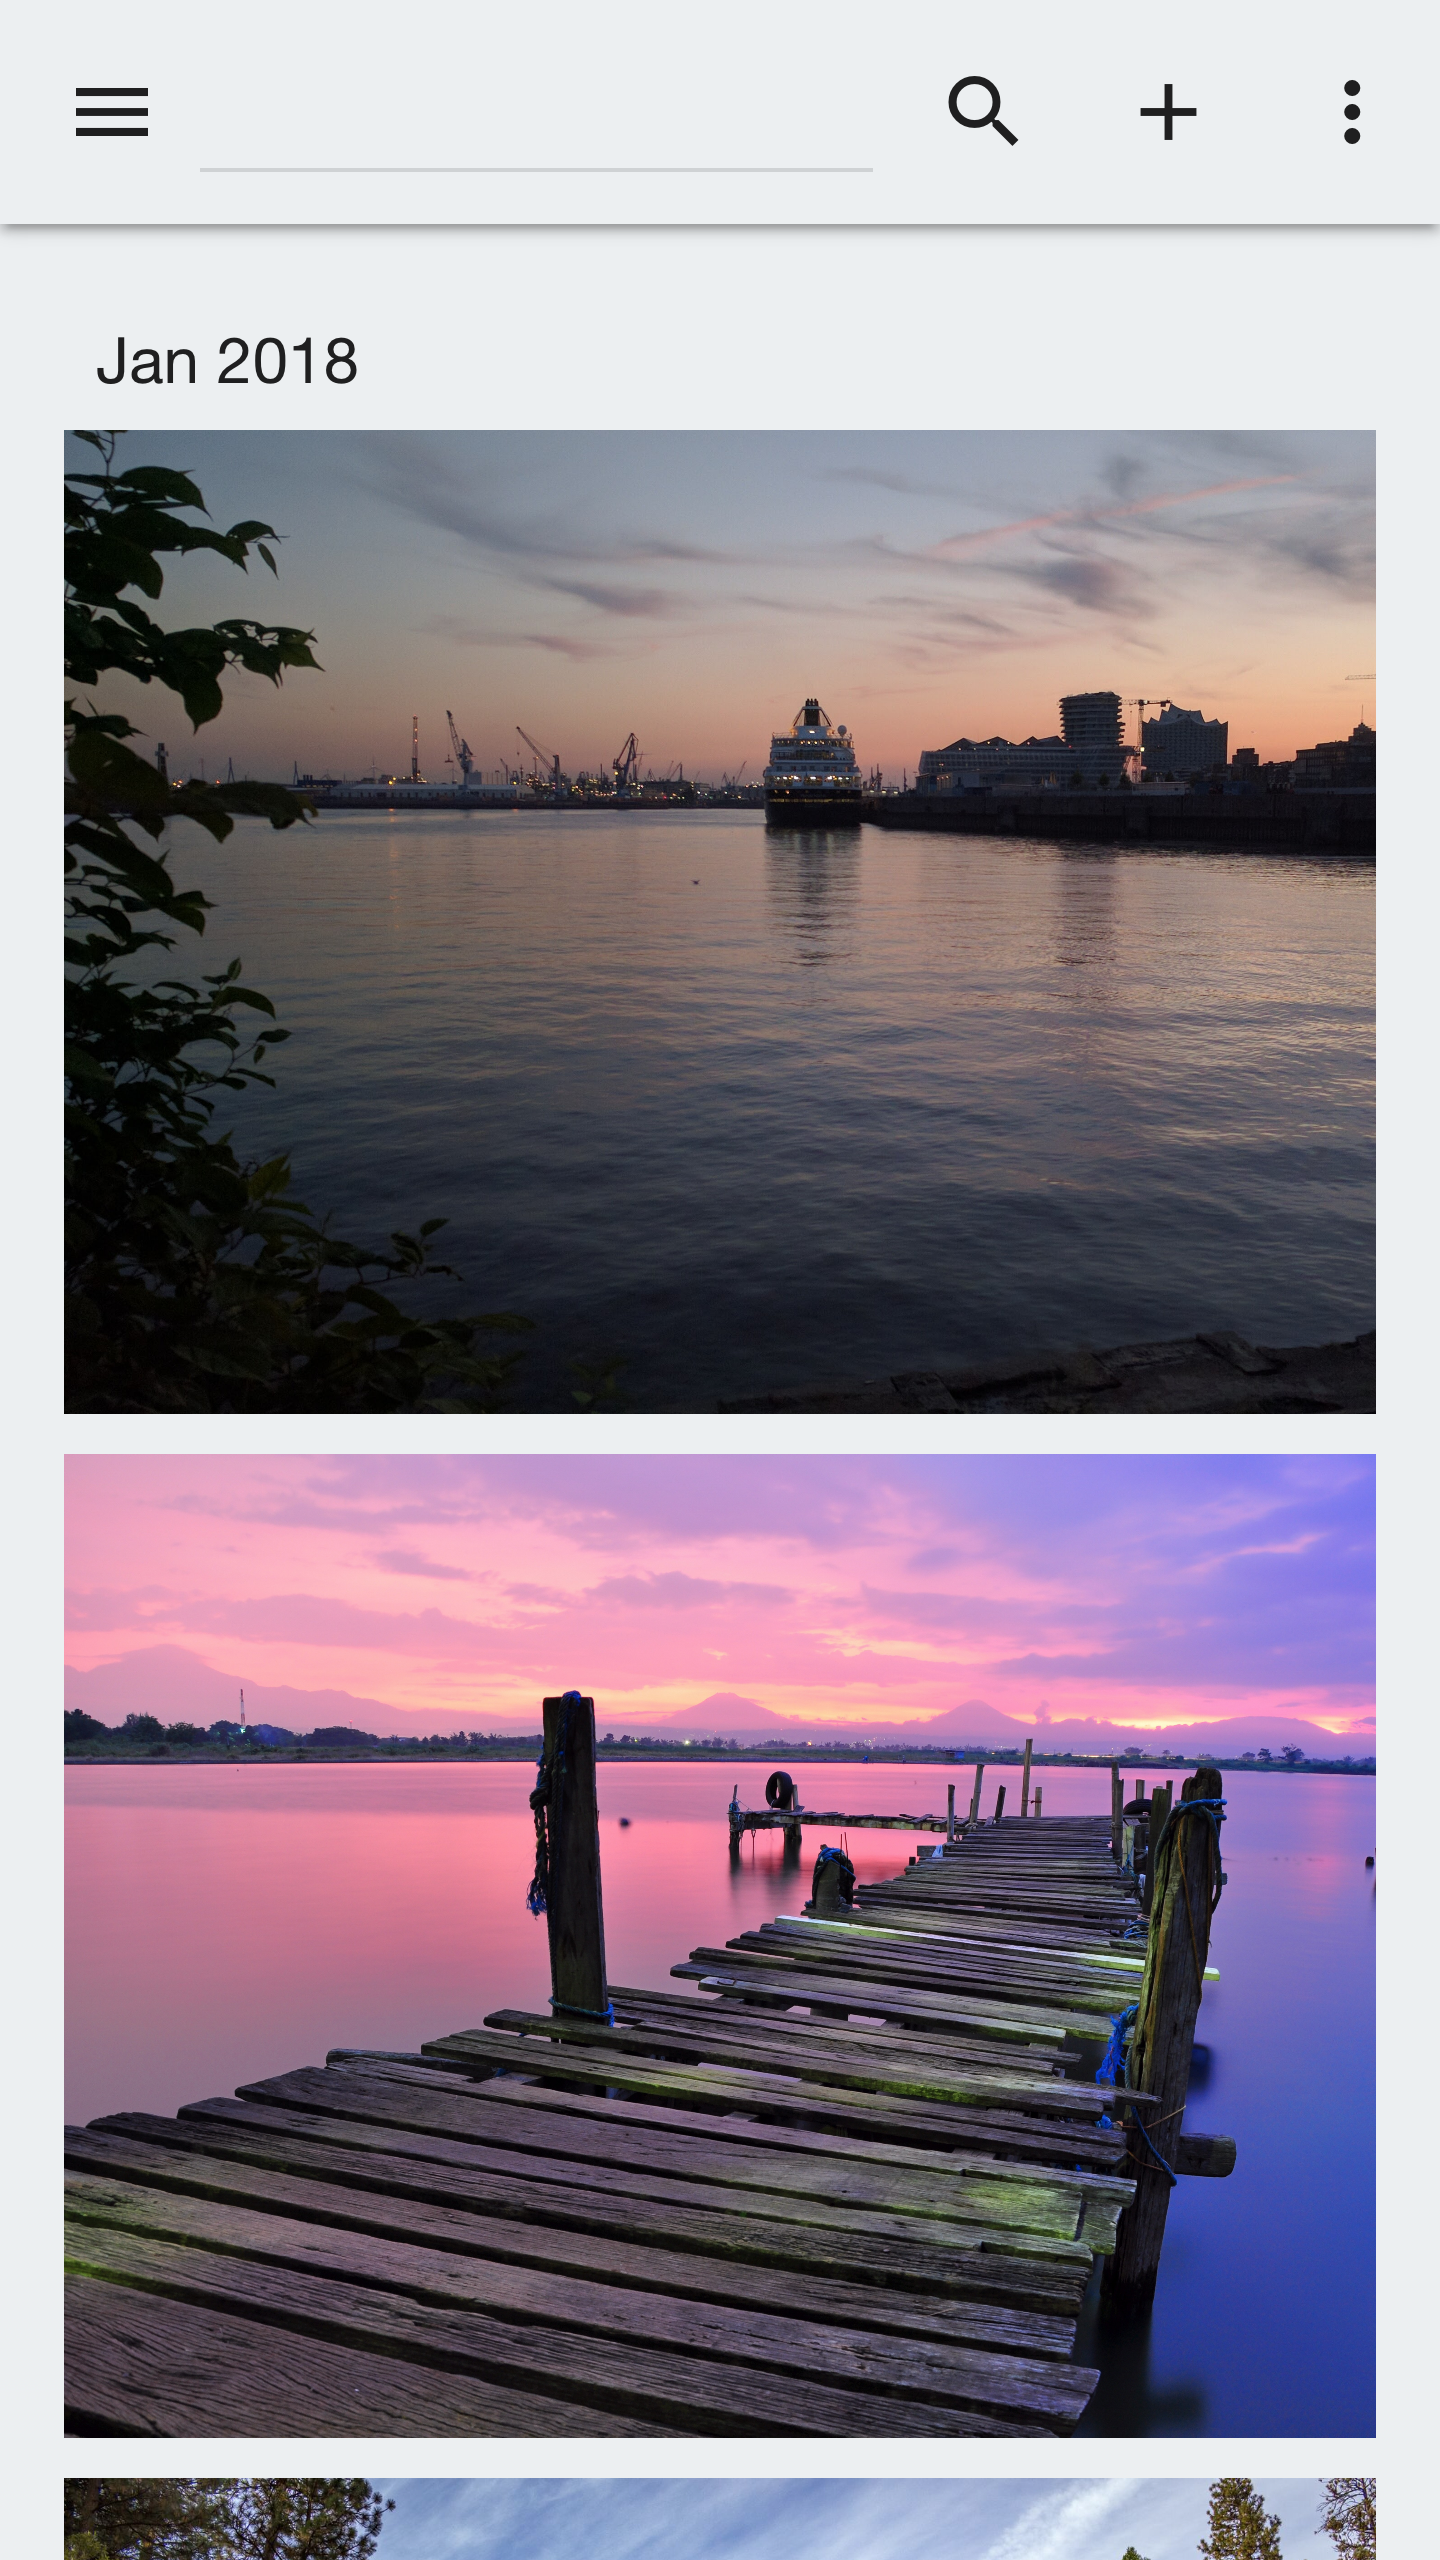
\includegraphics[width=0.5\textwidth]{images/gallery_small} 
\caption{Foto Gallerie Small}\label{fig:gallery_small}
\end{figure}

Die beiden oberen Entwürfe zeigen ebenfalls die Gruppierung der Fotos nach dem Erstellungsmonat (Anforderung \ref{sec:spec:photo_groups}) und die ein Suchfeld in der oberen Werkzeugleiste (Anforderung \ref{sec:spec:photo_search}). Die Eingabe eines Suchbegriffs führ instantan eine Suche durch, sobald mehr als 2 Zeichen eigegben werde. Das Ergebnis der Suche ist ebenfalls nach Erstellungsmonat gruppiert.

\section{Paginierung}

Für die Anforderung der Paginierung (\ref{sec:spec:pagination}) bietet die Andwendung dem Benutzer Paginierungs Links für jeweils 2 vorherige und kommende Fotobatches ( siehe \ref{fig:pagination}).

\begin{figure}[htp]     % h=here, t=top, b=bottom, p=page
\centering
\includegraphics[width=1.0\textwidth]{images/form_normal} 
\caption{Paginierung}\label{fig:pagination}
\end{figure}

\section{Foto Details}
Die Anforderung der Hauptansicht und Metadaten Betrachtung und Bearbeitung (\ref{sec:spec:photo_details}) ist in dem Visual Design  \ref{fig:form_normal} für die Bildschirmgröße Large abgebildet. Der Benutzer gelangt in die Foto Details Ansicht mit dem Klick auf ein entsprechendes Foto. 

Die Metadaten Ansicht wird mit dem Klick auf das Info Icon von rechts ausgeklappt und ist im Standardzustand nicht sichtbar. Das zentrierte Foto verschiebt sich entsprechend und skaliert im restlichen Bereich.

\begin{figure}[htp]     % h=here, t=top, b=bottom, p=page
\centering
\includegraphics[width=1.0\textwidth]{images/form_normal} 
\caption{Foto Details Normal}\label{fig:form_normal}
\end{figure}

Auf kleineren Geräten nimmt entweder das Foto (Abb. \ref{fig:details_small}) oder das Metadaten Formular den gesamten Platz ein (Abb. \ref{fig:form_small}). 

\begin{figure}[htp]     % h=here, t=top, b=bottom, p=page
\centering
\includegraphics[width=0.5\textwidth]{images/details_small} 
\caption{Foto Details Bild Small}\label{fig:details_small}
\end{figure}

\begin{figure}[htp]     % h=here, t=top, b=bottom, p=page
\centering
\includegraphics[width=0.5\textwidth]{images/form_small} 
\caption{Foto Details Metadaten Small}\label{fig:form_small}
\end{figure}

Die EXIF Kameradaten werden gesondert kategorisiert nach Erstellungsdatum, Kameraeinstellungen und Fotodimensionen mit einem entsprechenden Icon pro Kategorie angezeigt.

Die Abbildungen zeigen ebenfalls, dass das betrachtete Foto bei abnehmender Displaygröße proportionell herunterskaliert und immer auf dem Bildschirm zentriert wird (Anforderung \ref{sec:spec:photo_centering}).

Deweiteren sind über dem Foto blaue Pfeile für das Sliden zur nächsten bzw vorheriger Detailansicht eines Fotos in den oberen Entwürfen dargestellt. 
(Anforderunge \ref{sec:spec:photo_slider})

\chapter{Implementierung}

\section{Einleitung}

In Kapitel \ref{sec:zielsetzung} wurde als Zielsetzung bestimmt, dass diese grundlegende Problemstellungen bei der Implementierung einer komplexen clientseitigen Webanwendung betrachtet. Ferner hat \ref{sec:client_side_web_apps}gezeigt, dass hierfür eine komplette \textit{Ajax-Engine} an den Client über HTTP ausgeliefert werden muss. 

Für die Umsetzung dieser clientseitigen Architektur existiert eine Reihe von JavaScript Frameworks. Für die tatsächliche Implementierung der exemplarischen Fotoverwaltung Software verwendet diese Arbeit das AngularJS 1.x Framework. Dieses hält sich stark an die Konzepte objektorientierter Programmierung, liefert Bibliotheken zur Umsetzung des MVC Patterns aus Kapitel \ref{sec:architecture} und eine Reihe weitere für die Webbrowser Umgebung relevanter Werkzeuge wie URL Routing und DOM Rendering.

Für die Umsetzung des Benutzerinterface wird das mit AngularJS kompatible Angular Material Framework verwendet. Dieses bringt Material Farbenpaletten, graphische Elemente und Layout Abstraktion als \gls{ng-directive} auf der Grundlage des CSS Flexbox Layouts mit vordefinierten CSS Media Queries für die responsive Design Umsetzung.

\section{Layout}

Die Haupt- und Akzentpalette lassen sich bei dem Einbinden von Angular Material einmalig konfigurieren. Die UI Komponenten setzen das Theming oft automatisch um.
Dort wo es nicht passiert bzw. weitere Farbzustände für das Feedback bei Benutzerinteraktion benötigt werden, lassen sich über vorgegebene Parameter e.g \textit{md-primary}, \textit{md-raised} die Zustände setzen bzw. per Databinding umschalten.

Für das Navigationsmenü (Abb. \ref{fig:gallery_large}, links) wird die \gls{ng-directive} \textit{md-sidenav} verwendet. Die Komponente bietet Schnittstellen zum einklappen und ausklappen. Die Seitennavigation lässt sich parametrisiert entweder über den Inhalt legen oder kann den Inhalt wegschieben. Im Fall des Navigationsmenüs wird die erste Option verwendet. 

Die Untermenüs (Abb. \ref{fig:gallery_large}, oben) werden mit Hilfe des \textit{md-toolbar} Elements umgesetzt. Werkeuge, welche nicht auf die Leiste passen, lassen sich mit \textit{md-menu-content} in ein Kontexmenü verstecken, welches erst beim Klicken erscheint.

Angular Material bringt ebenfalls Container Abstraktionen für das Anordnen der Elemente. Es existieren Zeilen (\textit{layout="row"}), Spalten (\textit{layout="column"}) und Gridcontainer (\textit{md-grid}), welche Elemente horizontal bzw. vertikal anordnen. Dieses wird intern  mit Hilfe entsprechenden Flexbox Eigenschaften umgesetzt. Die Container sorgen automatisch dafür, dass die Größe der inneren Elemente für verschiedene Auflösungen skaliert wird. Alle Größenangaben werden prozentual zu der Größe des Elternelements gemacht, damit die responsive Eigenschaft gewahrt bleibt(siehe Abb. \ref{fig:layout_container}). 

\begin{figure}[htp]     % h=here, t=top, b=bottom, p=page
\centering
\includegraphics[width=1.0\textwidth]{images/layout_container} 
\caption{Layout Container. Quelle: material.angularjs.org}\label{fig:layout_container}
\end{figure}

Die Foto Galerie (Abb. \ref{fig:gallery_large}, mittig) besteht aus jeweils einem Zeilencontainer pro Monat der Aufnahme und zwei Zeilencontainer für die Monatsüberschrift sowie die Fotos selbst. Die Fotos werden wiederum in einem Gridcontainer gruppiert. 

Foto Details Metadaten (Abb. \ref{fig:form_normal}, rechts) befinden sich in einem von rechts ausklappbaren \textit{md-sidenav} Element. Es schiebt den Inhalt mit der Großansicht des Fotos weg und verdrängt es komplett auf kleinen Geräten. Die \textit{md-input} Formularfelder selbst lassen sich einer Spalte als Zeilen anordnen.

Das Foto (Abb. \ref{fig:form_normal}, links) wird mit Hilfe der Flexbox \textit{justify-content} Eigenschaft zentriert. In Angular Material wird dies über den Parameter \textit{layout-align="center center"} auf dem Wrapper Container erreicht. Damit das Foto aber auch korrekt proportional zu seinen eigentlichen Dimensionen skaliert, müssen alle weiteren Elterncontainer des Image Elements 100\% ihrer verfügbaren Breite und Höhe einnehmen. Hierfür sorgt die Eigenschaft \textit{layout-fill}.

\section{Grund Setup}
\label{sec:grund_setup}

Um die \textit{Ajax-Engine} zu bündeln, kommt \gls{webpack} zum Einsatz. Dieses erlaubt das Zusammenbauen mehrerer öffentlicher (vendor) und eigener JavaScript Module zu wenigen Buildfiles, welche bequem im Hauptmarkup eingebunden werden. Zudem wird dadurch ermöglicht, moderne JavaScript Syntax (e.g \gls{es2016}) durch Code Preprocessing durch sog. Transpiler, zu verwenden. Ein solcher Transpiler wandelt z.B. einen modernen JavaScript Standard in einen ursprünglichen Standard, welcher von den Zielbrowsern der Anwendung bereits implementiert wurde, um.

Das Resultat eines solchen Builds ist eine einzige HTML Seite \textit{index.html}, die der Benutzer am Ende ausgeliefert bekommt. Die Index Seite bettet wiederum nur zwei zusammengebaute Scripte aus allen bestehenden ein - \textit{index.bundle.css} und \textit{index.bundle.js}. Diese sind entsprechend für das gesamte Layout und die gesamte Business Logik der Anwendung verantwortlich (siehe \ref{lst:index_html}).

\begin{listing}[H]
\begin{minted}{html}
<!doctype html>

<head>
  <title>Pika</title>
</head>
<body ng-app="pika">
...

<script src="build/vendor.bundle.js"></script>
<script src="build/index.bundle.js"></script>
</body>
</html>

\end{minted}
\caption{index.html}
\label{lst:index_html}
\end{listing}

\gls{webpack} setzt auf das in \textit{ES2015} eingeführte \textit{Modules}Feature auf. Hierbei wird ein Entryscript in der \gls{webpack} Konfigurationsdatei deklariert. (ähnlich dem Main File eines herkömmlichen Programms). \gls{webpack} durchläuft beim Build jedes darin importierte File rekursiv und lässt es anhand weiterer deklarierter Regeln durch entsprechende Präprozessoren verarbeiten. Sowohl Stylesheets als auch Skripte werden so verarbeitet. Der Output dieser Präprozessoren wird am Ende, wie in Listing \ref{lst:index_html} abgebildet, zu einzelnen Files gebündelt.

In Listing \ref{lst:webpack_config} ist ein Auszug aus der \textit{Pika} Build Konfiguration zum Transpilieren von \textit{ES2016} JavaScript Standard zu \textit{ES5} Standard mit Hilfe des \textit{babel-loader}, sowie von \gls{sass} zu \textit{CSS} mit Hilfe des \textit{sass-loader} dargestellt.

\begin{listing}[H]
\begin{minted}{javascript}
{
  entry: {
    index: ['./index.js']
  },
  module: {
    rules: [
      {test: /\.scss$/, use: ['sass-loader']},
      {test: /\.js$/, use: ['babel-loader']}
    ]
  }
}
\end{minted}
\caption{webpack.config.js}
\label{lst:webpack_config}
\end{listing}

Für diese Applikation werden insgesamt folgende Regeln deklariert:

\begin{itemize}
 \item Herkömmliche CSS Bündelung aus anderen Paketen
 \item Statische Assets Einbindung und Fingerprinting für besseres Browsercaching
 \item Präprozessing von \gls{es2016} zu \textit{ES5} für moderne JavaScript Features, e.g. Klassen, Modularisierung, Arrow Functions, Parameter Destructuring, Promises   
 \item Präprozessing von \gls{sass} zu \textit{CSS} für erweitertes Stylesheet Tooling, wie Schachtelung, Vererbung, Variablen Verwendung
 \item Präprozessing durch \gls{pug} (ehemal. \textit{Jade}) Templates zu HTML für bessere Markup Lesbarkeit
 \item Extrahierung des separaten \textit{CSS} Bundles
 \item Trennung von Vendor und Applikation Codes in einzelne Bundles
\end{itemize}

Wie bereits oben erwähnt, bekommt der Benutzer eine einzelne Seite mit den gebündelten Skripten ausgeliefert. Der tatsächliche Inhalt der Applikation wird also erst durch das Bundle Skript auf dem Client erzeugt. Hierfür muss das AngularJS Framework wissen, welcher Platzhalter im DOM das Ziel des clientseitigen Renderings darstellen soll.  

Listing \ref{lst:index_html} zeigt, dass der \textit{body} Tag hierfür mit dem entsprechenden Attribut \textit{ng-app="pika"} markiert worden ist. Man spricht hier auch von einer \gls{ng-directive}. Damit AngularJS die Kontrolle über den Inhalt des \textit{body} Tags übernehmen kann, ist schlussendlich der folgende Aufruf im \textit{index.js} File notwendig. 

\begin{listing}[H]
\begin{minted}{javascript}
  import angular from 'angular';
  angular.module('pika', [ 
    //list of submodules 
  ])
\end{minted}
\end{listing}

\section{Routing}
\label{sec:routing}

Da Pika immer noch eine Webanwendung ist und im Browser ausgeführt wird, erwarten Benutzer, dass das Navigieren zwischen einzelnen Bereichen der Applikation mit einer Veränderung der URL in der Adresszeile des Browsers einhergeht. Ebenfalls soll es möglich sein zu einem bestimmten Bereich zu gelangen, indem man eine URL direkt in die Adresszeile des Browsers eingibt.

In \ref{sec:client_server} wurde jedoch erläutert, dass mit einer neuen Adresseingabe auch eine separate HTTP Anfrage verbunden ist. AngularJS bietet daher ein Routing Mechanismus an, welcher das Standardverhalten der Browser bei Adresseingaben kapert. 

URL Adresseingaben gehen zunächst durch den AngularJS Router in dem Client Code. Stellt dieser eine Adresse fest, welche in der Routingkonfiguration festgelegt wurde, so wird ein entsprechender Controller aufgerufen und seine Ausgabe in dem Hauptlayoutplatzhalter gerendert. 


\begin{listing}[H]
\begin{minted}{html}
<body ng-app="pika" layout="row" layout-fill>
<div layout="column" layout-fill ng-cloak="">
  <side-menu />
  <ui-view role="main" layout="column" layout-fill></ui-view>
</div>
</body>
\end{minted}
\caption{Hauptlayout}
\label{lst:main_layout}
\end{listing}

Listing \ref{lst:main_layout} zeigt den restlichen Inhalt der \textit{index.html}Datei. Entscheidend ist die Direktive \textit{ng-app="pika"}. Sie sorgt dafür, dass das in \textit{index.js} (\ref{lst:module_build}) deklarierte Angular Hauptmodul das Rendering des Inhalts hier übernehmen kann.

Der Inhalt der Anwendung besteht aus den Direktiven für das Seitenmenü (\textit{side-menu} ) und dem jeweiligen Inhalt des Routers (\textit{ui-view}). 

Letztendlich braucht das AngularJS Hauptmodul eine Konfiguration für das Routing von URLs zu den jeweiligen Hauptkontrollern der Applikation. Listing \ref{lst:routing_config} zeigt einen Auszug dieser Konfiguration. In dieser Arbeit wird ein 3rd Party Router, namens \textit{UI-Router} verwendet. (Der Standardrouter ist bereits für den exemplarischen Anwendungsfall dieser Arbeit sehr eingeschränkt. Die Notwendigkeit für den UI-Router wird im weiteren Verlauf deutlich).

\begin{listing}[H]
\begin{minted}{javascript}
import photosTemplate from './photos/index.jade';
import photoDetailTemplate from './photo-detail/index.jade';

function routesConfig($stateProvider, $urlRouterProvider) {
  $stateProvider
    .state('photos', {
      url: '/photos/:page?search',
      template: photosTemplate,
      controller: 'photosController',
      controllerAs: '$ctrl',
      resolve: { authenticate: authenticate }
    })
    .state('photo-detail', {
      url: '/photo-detail/:id',
      template: photoDetailTemplate,
      controller: 'photoDetailController',
      controllerAs: '$ctrl',
      resolve: { authenticate: authenticate }
    });
}

\end{minted}
\caption{routes.js}
\label{lst:routing_config}
\end{listing}

Die obige Konfiguration definiert folgendes Verhalten:
Die Adresseingabe von \textit{https://pika.cloud/photos?page=7} führt zum Instanziieren des \textit{PhotosController}. Dieser rendert die Seite 7 der Fotogalerie in den \textit{ui-view}. Ein Klick auf den Link hinter der Miniansicht eines Bildes ruft die URL \textit{https://pika.cloud/photo-details/p13tr3} auf und sorgt entsprechend dafür, dass der \textit{PhotoDetailController} die Großansicht des Fotos mit der ID  \textit{p13tr3} rendert.

\section{Projekt Struktur}
\label{sec:project_structure}

Die Analyse der Aufgabestellung für diese Anwendung im Kapitel Design ergab die Hauptdomainbereiche -  Authentifizierung und Session Handling (\textit{session}), Menünavigation (\textit{side-menu}), Foto Galerie und Suche (\textit{photos}), Detail Fotoansicht und Metadateneingabe (\textit{photo-detail}). Entsprechend dieser Domainbereiche wird die Modularisierung vorgenommen.

\subsection{Verzeichnis Struktur}

In zahlreichen Einstiegs Quellen für Organisation von JavaScript Projekten, findet man eine Bündelung nach Funktionsverantwortung der Komponenten im Angular Framework vor. So werden etwa Controller, Direktiven, Factories, Services in einzelnen Unterverzeichnissen organisiert. Dieser Aufbau hat den Nachteil, dass nicht sofort ersichtlich wird, wo sich der Applikationscode einer bestimmten Domain befindet, da er nun auf verschieden Orte verteilt ist. 

Pika verwendet daher eine Gliederung der Verzeichnisse nach ihrer Domain. Diese Praxis wird unter JavaScript Entwicklern favorisiert \footnote{https://stackoverflow.com/questions/18542353/angularjs-folder-structure} und etwa in \cite{Kukic:2014} detailliert dargestellt. Es ergibt sich daher die Verzeichnis Struktur aus Listing \ref{lst:directorty_structure}.


\begin{listing}[H]
\begin{minted}{bash}
# Detail Fotoansicht und Metadateneingabe 
|-- photo-detail 
|   |-- controller.js
|   |-- form-component.js
|   |-- form.jade
|   |-- index.jade
|   |-- index.js
|   |-- index.scss
|   |-- toolbar-component.js
|   `-- toolbar.jade

# Foto Gallery und Suche
|-- photos
|   |-- client.js
|   |-- controller.js
|   |-- gallery.js
|   |-- index.jade
|   |-- index.js
|   |-- index.scss
|   |-- toolbar-component.js
|   `-- toolbar.jade

# Authentifizierung und Session Handling
|-- session
|   |-- controller.js
|   |-- index.js
|   `-- session.js

# Menünavigation
|-- side-menu
|   |-- index.jade
|   |-- index.js
|   `-- index.scss
|-- http-interceptor.js

# Übergreifender Code
|-- index.js
|-- index.scss
|-- routes.js
`-- theming.js
\end{minted}
\caption{Directory Structure}
\label{lst:directorty_structure}
\end{listing}

\subsection{Modul Struktur}

Entsprechend der Domain Aufteilung lässt sich also jeder einzelne Bereich als ein einzelnes Angular Modul abbilden. Hierbei exportiert jedes einzelne Modul seine eigene Angular API Deklaration (siehe \ref{lst:module_export}). Diese Exports werden schließlich im dem \textit{index.js} File an das \textit{Pika} Hauptmodul übergeben ( siehe \ref{lst:module_build}).


\begin{listing}[H]
\begin{minted}{javascript}
//photos/index.js
import angular from 'angular';

import client from './client';
import gallery from './gallery';
import controller from './controller';
import toolbarComponent from './toolbar-component.js';

export default angular.module('pika.photos', [
  client.name,
  gallery.name,
  controller.name,
  toolbarComponent.name
]);
 
\end{minted}
\caption{Modul Export}
\label{lst:module_export}
\end{listing}

\begin{listing}[H]
\begin{minted}{javascript}
//index.js
import session from './session';
import sideMenu from './side-menu';
import photos from './photos';
import photoDetail from './photo-detail';

angular.module('pika', [
  'ui.router',
  'ngMaterial',
  'ngFileUpload',
  sideMenu.name,
  session.name,
  photos.name,
  photoDetail.name
])
\end{minted}
\caption{Modul Zusammenbau}
\label{lst:module_build}
\end{listing}

\subsection{Komponenten Struktur}

Kapitel \ref{sec:architecture} erläutert das Paradigma der clientseitigen Javascript MVC Frameworks. Es liegt darin einzelne Komponenten für Teilbereiche des HTML DOMs zu erstellen. Die Komponente nimmt alle Benutzerinteraktion in diesem Teilbereich entgegen, speichert und rendert dessen Zustand. 

Sie besteht aus mehreren weiteren Einheiten - einem View, einem Controller und einem bist mehreren Models. In dieser Arbeit nimmt der Controller, wie am Ende von  Kapitel \ref{sec:architecture} geschildert eine Presenter Rolle ein. D.h. er speichert nicht nur die Rohdaten für die Darstellung, sondern exakt den Zustand des Benutzerinterfaces. 

Betrachtet an dem Prozess der Fotogalerie Darstellung bedeutet es beispielsweise, dass der entsprechende \textit{PhotosController} die Daten exakt in der Form speichert, wie diese betrachtet werden. Die Darstellung der Fotogalerie ist nach Monat der Aufnahme gruppiert, die Rohdaten werden aber üblicherweise von einer Serverschnittselle als sortierte Liste zurückkommen. Es ist demnach die Aufgabe des Controllers in der Presenter Rolle, die Daten aus einer Liste gruppiert nach Aufnahme Monat abzulegen. Dafür kann er natürlich weitere Model Services hinzuziehen. Das View Markup bleibt somit sehr schlicht. Dieses Vorgehen ergibt eine maximale Trennung von visueller Darstellung und Applikationslogik.

Komponenten in Angular können entweder durch URL Routing in einem Platzhalter ausgetauscht werden (siehe \ref{sec:routing}) oder direkt durch eine Angular Direktive als eine Art Custom HTML Tag instanziiert werden, falls sich ihr Verhalten nicht auf die URL Änderung auswirken muss. 

Für diese Arbeit ergibt sich folgende generelle Komponenten Gliederung:

\begin{itemize}
\item Die vier Hauptdomainbereiche - \textit{session}, \textit{side-menu}, \textit{photos}, \textit{photo-details} - bilden entsprechende Komponenten und bestehen aus einem Hauptcontroller und einem zugehörigen Markup Template in \gls{pug} syntax (mit Ausnahme von \textit{session}). 
\item Photos- und PhotoDetails Controller werden über URL Routing angesprochen
\item Die Hauptbereiche besitzen weitere Komponenten Gliederungen, wie PhotoToolbar, PhotoDetails Toolbar, PhotoForm. Sie werden als Direktiven im Markup initialisiert.
\end{itemize}

\section{Session Handling}

\subsection{Grundverfahren}
\label{sec:session_handling_basics}

Kapitel \ref{sec:spec:authentication} definiert die Anforderung zur Benutzerauthentifizierung. Die Grundvorgehensweise dabei schildert sich wie folgt:

\begin{itemize}
  \item Der Benutzer gibt seine Anmeldedaten beim initialen Aufruf der Anwendung ein.
  \item Die Anmeldedaten werden auf dem Server validiert.
  \item Nach positiver Prüfung erhält der Benutzer einen Session Token.
  \item Der Client speichert den Session Token permanent ab.
  \item Der Session Token wird mit jeder weiteren Anfrage an den Server gesendet. 
\end{itemize}

Das obige Vorgehen liefert den Grundsatz einer Lösung auf das in Kapitel \ref{sec:client_server} geschilderte Problem der Zustandsbehaftung in dem zustandslosen HTTP Protokoll. Jede HTTP Anfrage erhält durch die obige Technik schließlich einen eindeutigen Session Token, über den der Server den Benutzer authentifizieren kann. 

Für die konkrete Implementierung existiert eine Reihe von Verfahren. Die einfachste Variante nutzt den Standard Cookie Mechanismus von HTTP, um den Session Token zu speichern. Wenn ein solcher Cookie vom Server gesetzt wurde, ist kein weiterer Client Code erforderlich, um diesen mit nachfolgenden Anfragen zu senden. Folglich ist es auch die ursprüngliche und einzige Variante, um rein serverseitige Webanwendungen zu authentifizieren.

Die Cookie Authentifizierung bietet allerdings die meiste Angriffsoberfläche. Aus diesem Grund verwenden eigen implementierte Webclients in aller Regel einen separaten Mechanismus. Der Standard JWT taucht oft in Zusammenhang von Authentifizierung von Single Page Applikationen auf. Tatsächlich spezifiziert JWT nur den Aufbau- und Verifizierungsmechanismus der Session Token. 

Für den tatsächlichen Authentifizierung Flow bietet es lediglich Richtlinien an. In einfacher Form benötigt der Client kein Wissen darüber, welche Art von Token Standard auf dem Server verwendet wurde. Daher zeigt diese Arbeit die Implementierung eines Authentifizierungsverfahren, welches einer solchen Richtlinie aus dem JWT Standard folgt. 

\subsection{Authentifizierung}

Den Aufruf der Root URL bearbeitet die \textit{SessionController\#index} Methode und rendert das Login Formular, wenn der Benutzer nicht eingeloggt ist (siehe \ref{lst:session_handling}).

Die \textit{SessionController\#create} Methode nimmt die Anmeldedaten aus dem Login Formular entgegen. Daraufhin sendet der Controller \textit{POST '/api/session-token'} mit den Benutzereingaben an den Server. Sollte die Eingabe falsch sein, wird die Fehlermeldung aus der Antwort in einer Instanzvariable des Controllers abgelegt und per \gls{databinding} im Formular gerendert. Die gültige Antwort des Servers enthält ein JSON Objekt mit den Daten des gegenwärtigen Users inklusive des JWT Session Tokens. 

Diese Daten müssen nun permanent abgelegt werden. Diese Aufgaben übernimmt das \textit{Session} Objekt. Der \textit{SessionController} leitet die Daten des gegenwärtigen Users an die \textit{Session\#authorize} Methode weiter. Darauf legt das Session Objekt diese über den \gls{localstorage} Mechanismus des Browsers ab. 

Beim erneuten Instanziieren des Session Objekts liest dessen Konstruktor das Token aus dem LocalStorage. Wird der \textit{SessionController\#index} erneut aufgerufen, prüft der \textit{SessionController} über \textit{Session\#isAuthenticated}, ob ein \textit{User} Objekt bekannt ist und übergibt das Rendering an den \textit{PhotosController}. Dies wird über die Router Schnittstelle \textit{this.\$state.go('photos')} erreicht. Der Befehl verändert die Adresszeile des Browsers auf die unter dem  \textit{photos} Schlüssel konfigurierte URL. Ebenfalls unter diesem Schlüssel in der Routerkonfiguration
wird festgelegt, dass der \textit{PhotosController} für die Navigation auf die obige URL zuständig ist. Angular sorgt dafür, dass der entsprechende Controller instanziiert wird und das Rendering übernimmt. Der Benutzer ist somit eingeloggt und sieht die Fotogalerie.

\begin{listing}[H]
\begin{minted}{javascript}
//session/controller.js
class SessionController {
  /** @ngInject */
  constructor($state, $http, session) {
    //...
  }

  index() {
    if (this.session.isAuthenticated()) {
      return this.$state.go('photos')
    }
  }

  create() {
    const _this = this;
    this.$http.post('/api/session-token', this.user)
    .then((response) => {
      _this.session.authenticate(response.data);
      _this.$state.go('photos');
    });
  }
}

export default angular.module('session.controller', [])
  .controller('sessionController', SessionController)

//session/session.js
class Session {

  constructor() {
    this.user = JSON.parse(localStorage.getItem('user')) || {};
  }

  authenticate(user) {
    this.user = user;
    localStorage.setItem('user', JSON.stringify(user));
  }

  isAuthenticated() {
    return !!this.user.token;
  }
}

export default angular.module('session.session', [])
  .service('session', Session)

\end{minted}
\caption{Session Handling}
\label{lst:session_handling}
\end{listing}

\subsection{Autorisierung}

Nach dem die erfolgreiche Authentifizierung des Users abgeschlossen ist, müssen einzelne Bereiche der Applikation nur für eingeloggte Nutzer autorisiert werden. Hierfür muss das Session Objekt für andere Komponenten im System verfügbar gemacht werden. 

Solche Abhängigkeiten werden in AngularJS über das \gls{di} Mechanismus aufgelöst. Der DI Con­tai­ner kümmert sich um die Instanziierung aller registrierten Objekte. Es kann hier festgelegt werden, ob eine Abhängigkeit nur ein Mal pro Modul als \gls{ng-service} verfügbar ist oder jedes Mal neu mit Hilfe einer \gls{ng-factory} instanziiert wird, wenn sie gebraucht wird. 
Die \textit{Session} Klasse wird als Service registriert, da dessen Instanz mit den User Daten über alle anfordernden Komponenten einmalig verfügbar sein muss. 

Eine Stelle, wo der authentifizierte Zustand geprüft wird, ist der Router. Alle Routes im System müssen den Benutzer zurück auf das Login Formular weiterleiten, wenn dieser nicht eingeloggt ist (siehe \ref{lst:route_authorization}).

\begin{listing}[H]
\begin{minted}{javascript}
//routes.js
function routesConfig($stateProvider, $urlRouterProvider) {
  $stateProvider
  // ...
    .state('photos', {
      url: '/photos/:page?search',
      template: photosTemplate,
      controller: 'photosController',
      controllerAs: '$ctrl',
      resolve: { authenticate: authenticate }
    })
  // ... 
}

function authenticate($q, $state, $timeout, session) {
  if (session.isAuthenticated()) {
    return $q.when();
  }

  $timeout(function() {
    $state.go('session');
  })

  return $q.reject();
}

\end{minted}
\caption{Route Autorisierung}
\label{lst:route_authorization}
\end{listing}

Über das \textit{resolve} Keyword lässt sich in der Router Konfiguration eine \textit{authenticate} Funktion anhängen. Diese wird immer aufgerufen, wenn eine Routeänderung auf die entsprechende Route passiert. Der Rückgabewert dieser Funktion - ein erfolgreich/nicht erfolgreich aufgelöstes Promise Objekt - bestimmt darüber, ob die Route Änderung wirklich durchgeführt werden darf.

Diese Entscheidung kann die \textit{authenticate} Funktion einfach treffen, indem es die API des injecteten Session Objektes \textit{session.isAuthenticated()} in Anspruch nimmt.

Das oben beschriebene Verfahren der Route Autorisierung ist offensichtlich keine Sicherheitsmaßnahme, da das Ganze in dem Client Code passiert. Es dient, wie angedeutet, lediglich der notwendigen User Experience - der User soll immer auf das Login Formular umgeleitet werden, falls nicht richtig autorisiert. 

Wie in Kapitel \ref{sec:session_handling_basics} geschildert, muss ein Server jede HTTP Anfrage auf das valide Session Token prüfen, da diese auch ohne des originalen Webclients von einem potentiellen Angreifer durchgeführt werden können. Das Session Objekt muss demnach bei allen HTTP Aufrufen bekannt sein. 

Angular bringt einen HTTP Client mit, welcher lediglich einen bequemeren Wrapper über die native Browser \textit{fetch} API darstellt. Über einen sog. \textit{HTTP Interceptor} lässt sich das Setzen des nötigen Autorisierungheaders einmalig konfigurieren (siehe \ref{lst:http_interceptor}).

\begin{listing}[H]
\begin{minted}{javascript}

//http-interceptor.js
export default function (session) {
  return {
    request: (config) => {
      if (session.isAuthenticated()) {
        config.headers.Authorization = `Bearer ${session.user.token}`;
      }
      return config;
    }
  };
};

\end{minted}
\caption{HTTP Interceptor}
\label{lst:http_interceptor}
\end{listing}

Die Abhängigkeit zu dem HTTP Client lässt sich über den von Angular mitgelieferten DI Container auflösen. Nach der korrekten Registrierung des HTTP Interceptor muss bei der Benutzung des Client nichts weiter beachtet werden (Siehe \ref{lst:http_client}).

\begin{listing}[H]
\begin{minted}{javascript}

//photos-client.js
class PhotosClient {
  constructor($http {
    this.$http = $http;
  }

  // ...

  findById(id) {
    return this.$http.get(`/api/photos/${id}`);
  }

  // ...
}  

\end{minted}
\caption{HTTP Client Verwendung}
\label{lst:http_client}
\end{listing} 

\section{Menüführung}

In Kapitel \ref{sec:des:navigation_menu} wurde ein Seitenmenü für die Hauptnavigation der Applikation und jeweils ein Untermenü für die Unterbereiche, wie die Galerieansicht oder Photo Detail Ansicht entworfen. Das Haupt Seitenmenü bleibt während des gesamten Nutzererlbnisses unverändert, während die Untermenüs sich je nach Kontext ändern können.

In Listing \ref{lst:main_layout} wurde der Lösungsansatz für die Menüführung bereits deutlich. Die Applikation benötigt ein Haupt Layout bzw. ein übergreifendes Frame. Dieses Frame enthält das Seitenmenü, dessen Komponente über die \gls{ng-directive} \textit{side-menu} im Markup initialisiert wird. Neben dem Seitenmenü ist ein Platzhalter für die Unterbereiche, dessen Inhalt von dem Router bestimmt wird. Die verschiedenen Kontext Untermenüs hingegen werden von der jeweiligen Hauptkomponente als Direktive in Markup eingebunden. Dies hat den Grund, dass der Kontext sich mit dem Wechsel in einen Unterbereich unterscheidet. Die Fotogalerie benötigt beispielsweise ein Suchfeld, während das die Detailansicht ein Button für das Anzeigen der Metadaten enthält.

Die Implementierung des Seitenmenüs gestaltet sich recht trivial. Der SideMenuController (siehe Listing \ref{lst:side_menu_controller}) initialisiert Menüeinträge. Es sind Lediglich Einträge mit Namen und URL Route zu dem Unterbereich. Der Controller muss somit nicht auf die Navigation selbst reagieren, da diese von dem Router übernommen wird.

\begin{listing}[H]
\begin{minted}{javascript}

import angular from 'angular';
import template from './index.jade';

class SideMenuController {

  /** @ngInject */
  constructor($mdSidenav) {
    this.$mdSidenav = $mdSidenav;
    this.initMenu();
    this.initAdminMenu();
  }

  initMenu() {
    this.menu = [
      {
        link: '/photos',
        title: 'Photos',
        icon: 'image',
      },
      {
        link: '/settings',
        title: 'Settings',
        icon: 'settings',
      },
      //...
    ];
  }

  close() {
    this.$mdSidenav('left').close();
  }
}

export default angular.module('pika.side-menu', [])
  .component('sideMenu', {
    template: template(),
    controller: SideMenuController,
    controllerAs: 'sideMenuController',
  });


\end{minted}
\caption{SideMenuController}
\label{lst:side_menu_controller}
\end{listing} 


\begin{listing}[H]
\begin{minted}{pug}

//side-menu/index.jade
md-sidenav.md-sidenav-left()
  // ...
  md-content
    md-list(flex='')
      md-list-item(ng-repeat='item in sideMenuController.menu')
        md-icon.blue_grey-400.material-icons.step {{item.icon}}
        p a(href='item.link')
            {{item.title}}
     
    md-button(ng-click='sideMenuController.close()', class='md-primary') 
      Close

\end{minted}
\caption{Side Menu View}
\label{lst:side_menu_view}
\end{listing} 

Das Verhalten des Seitenmenüs inklusive Ein- und Ausklappen Animation bringt die Angular \textit{mdSideNav} Komponente mit, welche schließlich im Markup erzeugt wird (siehe Listing \ref{lst:side_menu_view}). Paradoxerweise ist der SideMenuController nicht für das ausklappen des Seitenmenüs zuständig. Diese Aufgabe übernehmen die Kontextmenüs. Dies hat den einfachen Grund, dass der Ausklappregler sich in dem jeweiligen Kontextmenü links und nicht in dem Seitenmenü selbst befindet. Der Button zum ausklappen lässt sich ebenfalls in eine extra Komponente auslagern und in jede Kontext Toolbar integrieren. 

\section{Foto Galerie}
\label{sec:photo_gallery}

\subsection{Laden}

Die Fotogalerie ist ein Exempel für die Kommunikation über mehrere Controller und Wiederverwendbarkeit von Models. Denn die Einzelansicht des Fotos ist ebenfalls ein Art Galerie, da hier das Sliden zum nächsten und vorherigen Foto ermöglicht werden soll. Aus diesem Grund entsteht die Notwendigkeit das Laden von Fotos in Chunks an ein separates Model - die \textit{PhotosGallery} auszulagern. 

Die \textit{PhotosGallery} kann zwischen den \textit{PhotosController} und \textit{PhotoDetailsController} wiederverwendet werden. Sie speichert den aktuell geladenen Chunk an Fotos sowie das aktuell ausgewählte Foto. Navigiert der Benutzer auf die nächste Galerieseite oder will weiter als den letzte gecachte State in der PhotosGallery in der Detaiansicht der Photos sliden, wird der nächste Chunk geladen. Die beiden Controller und Views beobachten diese Änderung und stellen den neuen Zustand dar. Somit wird die Galerieansicht immer das entsprechende Detailphoto beinhalten, auch wen der Benutzer mehrere weitere Batches geladen hat.

Die Navigation zu \textit{\/photos} rendert die Foto Galerie. Dies übernimmt  \textit{PhotosController\#showPhotos}. Der Controller deklariert eine Abhängigkeit auf die \textit{PhotosGallery}, welche wiederum über den \textit{PhotosClient} den HTTP GET Aufruf an den Server durchführt. 

Die Antwort ist ein Array in \gls{json} Format von Foto Metadaten mit Titel, Beschreibung, diversen Kameraeinstellungen und der URL zu dem eigentlichen File. \gls{json} wird in JavaScript durch einen Aufruf von \textit{JSON.parse} direkt in ein Objekt umgewandelt. Der Angular HTTP Client macht es automatisch. Da die Darstellungslogik in den Controllern (Presentern) liegt, werden diese Rohdaten Objekte direkt als Models verwendet ohne extra Klassen dafür anzulegen. Die Foto Metadaten werden in der Instanzvariable \textit{photos} in der \textit{PhotosGallery} abgelegt. 


\begin{listing}[H]
\begin{minted}{javascript}

class PhotosController {
  /** @ngInject */
  constructor($scope, $stateParams, $state, photosGallery) {
    // ...
    this.photosGallery = photosGallery;
    this.showPhotos();
  }

  showPhots() {
    //...
    this.photosGallery.showPhotos(/**/);
  }
}

class PhotosGallery {
  /** @ngInject */
  constructor(photosClient) {
    this.client = photosClient;
    this.photos = [];
    // ...
  }
    
  showPhotos(params) {
    const self = this;
    //...
    return this.client.find(params).then(res => {
      self.photos = res.data.photos; 
      //...
      return self.photos;
    });
  }

}

\end{minted}
\caption{Photo Galerie}
\label{lst:photo_gallery}
\end{listing} 

\subsection{Gruppieren}

Nach dem die Fotos erfolgreich in dem \textit{PhotoGallery} Service geladen wurden, müssen die Rohdaten für die eigentliche Darstellung verarbeitet werden. Dieses Kapitel zeigt die weitere Verarbeitung exemplarisch anhand automatisch nach dem Monatsdatum gruppierter Darstellung der Fotos.

Diese Logik ist spezifisch für die Galerieansicht und wird im PhotosController angewendet. Die Gruppierung der Photos muss mit jeder Änderung des Arrays in der \textit{PhotoGallery} passieren. Der \textit{PhotosController} trägt sich hierfür als Watcher auf Änderungen des \textit{photos} Arrays im \textit{PhotoGallery} Service ein. 

Nach einer Änderung des \textit{photos} Arrays führt der Controller eine Grupperungsfunktion aus und legt das Endresultat in einer eigenen Instanzvariable ab. Der View rendert den Zustand der neuen Instanzvariable.

\begin{listing}[H]
\begin{minted}{javascript}

class PhotosController {
  /** @ngInject */
  constructor($scope, $stateParams, $state, photosGallery) {
    // ...
    this.photosGallery = photosGallery;
    this.photos = {};

    this.showPhotos();
    this.initWatchers();
  }

  initWatchers() {
    this.$scope.$watch(
      () => { return this.photosGallery.photos }, 
      this.filterPhotosByUploadMonth.bind(this)
    );
  }

  // reduce a key value list, of month to photos array
  // e.g
  // { 'Jan' => [ {id: 1, ... }, {id: 2, ...}, ... }]
  filterPhotosByUploadMonth(photos) {
    this.photos = photos.reduce((photosByMonth, photo) => {
      const uploadMonth = this.uploadMonth(photo);
      if (!photosByMonth[uploadMonth]) photosByMonth[uploadMonth] = [];

      photosByMonth[uploadMonth].push(photo);
      return photosByMonth;
    }, {});
  }
}

\end{minted}
\caption{Foto Gruppierung}
\label{lst:photo_group}
\end{listing} 

\subsection{Paginieren}

Für das laden von Fotos in Chunks wird in dem Benutzerinterface eine simple Paginierung verwendet. Es werden Links auf zwei vorherigen und folgenden Seiten mit jeweils 50 Bildern angezeigt. E.g. [5, 6, 7, 8, 9]. 

Das Laden des nächsten Chunks von Fotos passiert durch das Clicken des entsprechenden Page Links und wird in der Browser Adresszeile abgebildet. Es kann aber auch durch das Sliden zum nächsten/vorherigen Foto in der Detailansicht passieren. Somit ist wiederum der PhotoGallery Service für die Paginierung verantwortlich.

Der PhotosClient, über den letztendlich die Daten angefragt werden, akzeptiert einen \textit{page} Parameter, welchen er per HTTP Query Parameter wiederum an den Server senden kann. Basierend auf der aktuell angefragten Seite, generiert der \textit{PhotoGallery} Service ein Array aus Seitenzeilen in einer Instanzvariable nach jedem Laden eines Fotos Chunks. 

Die Paginierung geschieht folgender Weise:

\begin{itemize}
  \item Der Benutzer lädt die \textit{/photos} Url ohne \textit{page} Parameter
  \item Der \textit{PhotosGallery} Service lädt den Initialbatch \textit{1} mit 50 Fotos 
  \item Der \textit{PhotosGallery} Service generiert den ersten Bereich aus Seitenlinks [1,2,3,4,5]
  \item Der \textit{FotosController} rendert die Fotos und die Seitenlinks.
  \item Der Benutzer klickt auf einen der Links, e.g 5.
  \item Der \textit{PhotosController} nimmt die Aktion, mit dem Seitenparameter entgegen, sorgt darauf für eine Route Änderung, welche die Seitenzahl enthält, e.g. \textit{\/photos\/5}
  (Dieser Schritt ist notwendig, damit sich die Seitenzahl ebenfalls in der Adresszeile widerspiegelt und damit auch über die Adresszeile navigiert werden kann)
  \item Der \textit{PhotosController} wird durch den Router neu initialisiert, liest den \textit{page} Parameter aus dem Router, fordert \textit{PhotosGallery} auf den neuen Batch zu laden.
  \item Der \textit{PhotosGallery} Service fragt den entsprechenden Batch vom \textit{PhotosClient} an, legt den Batch in einer Instanzvariable ab, generiert neue Pagination Links.
\end{itemize}

\begin{listing}[H]
\begin{minted}{javascript}

class PhotosController {
  constructor(/**/) {
    //...
    this.showPhotos();
  }

  showPhotos() {
    const page = parseInt(this.$stateParams.page, 10)
    const search = this.$stateParams.search

    this.photosGallery.showPhotos({page, search});
  }

  // triggered on page link click
  showPage(page) {
    this.$state.go(
      'photos', 
      { page, search: this.photosGallery.search },
      { location: 'replace' }
    );
  }
}

class PhotoGallery {
  showPhotos(params) {
    //assign defaults in case no params passed
    const findParams = {
      search: params.search || this.search,
      page: params.page || this.currentPage
    }

    const self = this;
    return this.client.find(findParams).then(res => {
      self.pthotos = res.data.photos;
      self.totalSize = res.data.totalSize;
      self.currentPage = findParams.page;
      self.search = findParams.search;

      self.paginate();
      return self.photos;
    });
  }

  paginate() {
    let start = this.currentPage - 2;
    let end = start + 5;
    // ... handle edge cases ...
    this.pages = _.range(start, end);
  }
}

\end{minted}
\caption{Paginierung}
\label{lst:pagination}
\end{listing} 

\subsection{Rendering}
\label{sec:rendering}

Das Markup der Foto Galerie ist ein Logikfreies Rendering der oben erläuterten Datenstrukturen. Pro Monat der Aufnahmen wird eine GridList mit den Fotokacheln gerendert und unten auf der Seite eine Zeile mit den Paginierunglinks angehängt.
Pro Foto wird eine Grid Kachel \textit{md-grid-tile} erstellt. Das Foto selbst ist ein CSS \textit{background-image} Attribut der Kachel. Die Kachel erhält ebenfalls eine \textit{ng-click} Direktive mit entsprechender Aktion und Foto  ID, um bei einem Klick auf das Foto auf die Detailansicht zu gelangen.

\begin{listing}[H]
\begin{minted}{pug}

photos-toolbar

md-content()
  div(ng-repeat='(uploadMonth, photos) in $ctrl.photos')

    div {{uploadMonth}}

    md-grid-list()
      md-grid-tile(
        ng-repeat='photo in photos'
        ng-style="{ 'background-image': 'url(' + photo.src + ')'}"
        ng-click="$ctrl.showPhoto(photo._id)"
      )
        md-grid-tile-footer
          h3 {{photo.metadata.title}}
{}
  div(layout='row')
    md-button(
      ng-repeat='page in $ctrl.photosGallery.pages'
      ng-click='$ctrl.showPage(page)'
   ) {{page}}


\end{minted}
\caption{Foto Gallerie Markup}
\label{lst:photo_group_jade}
\end{listing} 

\section{Foto Suche}

Die Foto Suche verwendet für die Darstellung den exakt gleichen Code aus Kapitel \ref{sec:photo_gallery}. Die einzige Erweiterung, welche für die Suchefunktion notwendig ist, ist eine Weitergabe eines Suchbegriffes an den \textit{PhotoGallery} Service und wiederum an den HTTP Aufruf im \textit{PhotosClient}.

Das Suchfeld wird in die galeriespezifische Toolbar Platziert. Nach der Eingabe wird ein Route Änderung über den Angular Router erzwungen. Die Route führt wie in dem Standardfall auf den \textit{PhotosController}, enthält jedoch einen Suchbegriff in Route Parameter. e.g \textit{/photos?search=hamburg}. 

Der \textit{PhotosController} liest beim Laden der Fotos, wie in \ref{lst:pagination} gezeigt, durch die \textit{showPhotos} Methode zusätzlich den  
\textit{search} Parameter aus. Dieser wird dann an \textit{PhotoGellary.showPhotos} weitergereicht. 

Letzendlich ist die Aufgabe des Servers enttprechend ein gefiltertes Ergebnis zurückzugeben. Der Suchbegriff muss zusätzlich zwischengespeichert werden, damit die Paginierung den Suchfilter beachtet.

\section{Foto Details}
\label{sec:photo_details}

In Kapitel \ref{sec:rendering} wird erwähnt, dass jede Foto Kachel eine Click Aktion zugewiesen bekommt, welche zur der Detailansicht eines Fotos führt. Diese Aktion wird vom \textit{PhotosController} verarbeitet und ist eine triviale Routänderung auf den \textit{PhotoDetailsController} mit entsprechenden Photo ID Parameter in der URL. Die Routeänderung sorgt dafür, dass der \textit{PhotoDetailsController} neu instanziiert wird. Bei jedem Instanziieren lädt der \textit{PhotoDetailsController} das entsprechende Photo aus dem  Photo ID Parameter. Der \textit{PhotoDetailsController} verwendet ebenfalls wie der \textit{PhotoDetailsController} den \textit{PhotoGallery} Service, um die Daten für das einzelne Foto zu laden. 

Im Standardfall hat die PhotoGallery die Daten für das einzelne Foto bereits in dem \textit{photos} Array. Diese befinden sich dort aus der vorherigen Anfrage des \textit{PhotosController} für die Darstellung der Photoübersicht. Da ein Batch aus Fotos eine überschaubare Größe hat, reicht hier eine lineare Suche nach dem Eintrag mit des Fotos mit entsprechender ID. Das gefundene Foto Objekt inklusive der Foto Metadaten wird in der Instanzvariable \textit{currentPhoto} abgelegt und per Databinding gerendert. 

Die Anzeige der Metadaten ist hinter einer weiteren, von Rechts ausklappbaren Sidebar (siehe \ref{fig:form_normal}) versteckt. Editierbare Werte wie Title und Beschreibung werden in Formularfelder dargestellt. Ein bidirektionales Databinding kopiert die Benutzereingaben in die entsprechende Felder des \textit{currentPhoto} Objekts. 

Der PhotoDetails Controller registriert sich auf die \textit{onChanged } Events der Formularfelder und sendet nach einem kurzem Timeout die neuen bekannten Daten an den Server mit Hilfe des \textit{PhotoClient} Objektes. Somit ergibt sich ein sog. ``In Place Editing'' Benutzererlebnis.

\section{Foto Slider}
\label{sec:photo_slider}

Die Foto Detailansicht bittet gleichzeitig das Sliden zur Detailansicht des nächsten Fotos. Daher musst der \textit{PhotoGallery} Service Objekt ebenfalls den aktuellen Index in dem \textit{photos} Batch beim Laden der Photo Details (\ref{sec:photo_details}) speichern.

Grundsätzlich wird das Sliden zum nächsten bzw. vorherigen Foto durch ein Inkrementieren bzw. Dekrementieren des Indexes implentiert. Bei Indexänderung wird das entsprechende Foto in die \textit{currentPhoto} Variabe gelanden und gerendert.

Es fndet eine Ausnahmebehandlung statt, wenn der Index außerhalb der Grenzen des zwischengespeicherten Batches an Fotos wandert. Da die \textit{currentPage} Nummer auch gespeichert wird, kann an dieser Stelle der nächste/vorherige Batch an Fotos geladen werden. Die \textit{PhotoGallery\#showPhotos} Methode aus \ref{lst:pagination} kann hier wiederverwendet werden. An dieser Stelle wird der Grund für die Auslagerung der Gallery Funktion in einen separaten Service besonders deutlich.

Der folgende Pseudocode veranschaulicht das Verfahren unter Verzicht auf die Details der asynchronen JavaScript Programmierung.

\begin{listing}[H]
\begin{minted}{javascript}

class PhotoGallery {
  showPhotos(params) { /* ... */}

  next() {
    return this.slide(1);
  }

  prev() {
    return this.slide(-1);
  }


  slide(step = 1) {
    const nextIndex = this.currentIndex + step;
    const nextPage = this.currentPage + Math.sign(step);

    if (this.isIndexWithinPage(nextIndex)) {
      this.setIndex(nextIndex);
      return;
    }

    if (nextPage <= 0) {
      return;
    }

    this.showPhotos({ page: nextPage });
    // ... 
    // reset index to 0 (for next) or size-1 for (prev)  
  }

  isIndexWithinPage(index) {
    return index >= 0 && index < this.photos.length;
  }

   setIndex(index) {
    this.currentPhoto = this.photos[index];
    this.currentIndex = index;
  }
}

\end{minted}
\caption{Sliding}
\label{lst:sliding}
\end{listing} 

\chapter{Fazit und Ausblick}

\section{Fazit}

Die Arbeit schaute auf die historische Entwicklung des World Wide Webs vom klassischen Client-Server-Modell bis zur Entstehung immer mächtigerer Mechanismen für Webanwendungen, die eines reichhaltigeren Benutzererlebnises auf den Endgeräten bedürfen.

Für einen solchen potentiell an Benutzerinteraktionen reichen, nativ ähnlichen Client einer Webanwendung in Form einer Fotoverwaltungssoftware wurden charakteristische Anforderungen aufgestellt. Anhand der Analyse und Implementierung dieser Anforderungen wurden die konkreten Pro­b­le­ma­tiken des Software Designs eines solchen Clients im Detail verdeutlicht.

Es wurde gezeigt, wie eine solche Software on-the-fly an den Benutzer durch normale Webmechanismen ohne extra Installation ausgeliefert werden kann.
Ohne zur Implementierungzeit etwas über das Endgerät des Benutzers zu wissen, kann sich die realisierte Fotoverwaltungsapplikation an das tatsächliche Endgerät mit Hilfe von Responsive Webdesign anpassen.

Im Kontrast zur der oft üblichen Praktik der Anreicherung des Benutzererlebnisses mit Hilfe von einzelnen Skripten, wurde der Fokus der Arbeit darauf gelegt, die gewachsene Komplexität im Client durch saubere Trennung von Verantwortlichkeiten zu handhaben. Dabei entstanden einzelne Software-Komponente aus mehreren Entitäten für die jeweiligen Domain-Bereiche der Applikation. Zum einen wurde verdeutlicht, dass sich nun ein Bedarf für eine Kommunikation und Wiederverwendung der Logik zwischen einzelnen dieser Komponenten ergibt, und zum anderen wurde gezeigt, wie ein Anwendungszustand zwischen diesen Komponenten verwaltet werden kann.

\section{Ausblick}

Die Anforderung an Client-Server-Kommunikation wurde im Ansatz betrachtet. In großen Webanwendungen mit verschiedenen Endgeräten ergibt sich oft ein Bedarf an eine weit komplexere Datenschnittstelle mit Optionsparametern und Beziehungen zwischen einzelnen Datenstrukturen.

Für die Autorisierung und Authentifizierung wurde eine minimal hinreichende Lösung durch JWT Tokens aufgezeigt, welche zwar über den Browser-Standard-Cookie-Mechanismus hinausgeht, jedoch bei weitem nicht die Breite des Themas von Sicherheit in Webanwendungen erfasst. Zum Beispiel ergibt sich eine Fragestellung, wie Sicherheitstoken valide sein sollen und wie sie invalidiert werden. Ferner sind Webanwendungen meistens Mehrbenutzersysteme und bedürfen komplexerer Benutzer- und Rechtelogik.

Eine Thema, welches außer Acht gelassen wurde, ist die Testbarkeit von reichhaltigen Clients. In einer Single Page Webapplikation ergeben sich ebenfalls Besonderheiten im Gegensatz zur nativen Offline-Software wegen der Browserumgebung und des Simulierens der Client-Server-Kommunikation unter Test.

Webanwendungen haben den Vorteil einer on-the-fly Auslieferung und erlauben dem Benutzer, eine komplexe Software ohne eine lokale Installation zu benutzen. Sie haben allerdings Grenzen. Eine weitere Fragestellung ist, wie weit diese Grenzen reichen und welche Szenarien auch mit reichhaltigen Webanwendungen schwer bis gar nicht realisierbar sind.


\appendix


%--------------------- VERZEICHNISSE ----------------

\listoffigures % Abbildungsverzeichnis erzeugen
\listoflistings % Quellcodeverzeichnis erzeugen
\printglossaries

%--------------------- LITERATURLISTE ---------------
% Die Einträge sollen alphabetisch sortiert sein.

\bibliographystyle{dinat}
\bibliography{literature/index}

%--------------------- EIGENSTÄNDIGKEITSERKLÄRUNG ---------------
\clearpage\thispagestyle{empty}
\eigen  % im header definiert
%--------------------------------------- ENDE ------------------------------------
\end{document}
%%%%%%%%%%%%%%%%%%%%%%%%%%%%%%%%%%%%











